\documentclass[11pt,a4paper]{article}

% ---------------------------------------------------------------------------
% Attracting oscillations in sequential distributive multisite phosphorylation
%
% Author metadata: set the three macros below before submission.
% They are deliberately left blank in this version.
% ---------------------------------------------------------------------------
\newcommand{\PaperAuthor}{}
\newcommand{\PaperAffiliation}{}
\newcommand{\PaperDate}{17 September 2026}

\usepackage[T1]{fontenc}
\usepackage[utf8]{inputenc}
\usepackage{lmodern}
\usepackage{microtype}
\usepackage[a4paper,margin=1.05in]{geometry}
\usepackage{amsmath,amssymb,amsthm,mathtools}
\usepackage{booktabs}
\usepackage{array}
\usepackage{enumitem}
\usepackage{xcolor}
\usepackage{graphicx}
\usepackage{tikz}
\usetikzlibrary{arrows.meta,positioning,calc}
\usepackage[obeyspaces,spaces]{url}
\usepackage[numbers,sort&compress]{natbib}
\usepackage[colorlinks=true,linkcolor=blue!55!black,citecolor=blue!55!black,urlcolor=blue!55!black]{hyperref}
\hypersetup{pdftitle={Attracting oscillations in sequential distributive multisite phosphorylation},
  pdfkeywords={multisite phosphorylation, futile cycle, Hopf bifurcation, first Lyapunov coefficient, limit cycle, enzyme sequestration, quasi-steady-state approximation, computer-assisted proof, interval arithmetic, Lean}}

\DeclareUrlCommand\lean{\urlstyle{tt}}
\setlist{itemsep=2pt,topsep=3pt}
\setlength{\emergencystretch}{1.5em}
\graphicspath{{figures/}}

\theoremstyle{plain}
\newtheorem{theorem}{Theorem}[section]
\newtheorem{proposition}[theorem]{Proposition}
\newtheorem{lemma}[theorem]{Lemma}
\newtheorem{corollary}[theorem]{Corollary}
\theoremstyle{definition}
\newtheorem{definition}[theorem]{Definition}
\newtheorem{question}[theorem]{Question}
\theoremstyle{remark}
\newtheorem{remark}[theorem]{Remark}

\newcommand{\R}{\mathbb R}
\newcommand{\C}{\mathbb C}
\newcommand{\ii}{\mathrm i}
\newcommand{\T}{\mathsf T}
\newcommand{\cN}{\mathcal N}
\newcommand{\cP}{\mathcal P}
\newcommand{\ET}{E_{\mathrm T}}
\newcommand{\FT}{F_{\mathrm T}}
\newcommand{\ST}{S_{\mathrm T}}
\newcommand{\rA}{r_{\mathrm A}}
\newcommand{\omA}{\omega_{\mathrm A}}
\newcommand{\rH}{r_{\mathrm H}}
\newcommand{\omH}{\omega_{\mathrm H}}
\newcommand{\WA}{\mathsf A}
\newcommand{\WH}{\mathsf H}
\DeclareMathOperator{\diag}{diag}
\DeclareMathOperator{\Ree}{Re}
\DeclareMathOperator{\Imm}{Im}
\DeclareMathOperator{\rank}{rank}
\newcommand{\evC}{\textsf{C}}
\newcommand{\evI}{\textsf{I}}
\newcommand{\evK}{\textsf{K}}
\newcommand{\evN}{\textsf{N}}

\title{Attracting oscillations in sequential distributive\\ multisite phosphorylation:\\[2pt]
\large dynamic enzyme sequestration and what static elimination cannot see}
\author{\PaperAuthor\\[2pt]\small\PaperAffiliation}
\date{\PaperDate}

\begin{document}
\maketitle

\begin{abstract}
The sequential distributive $n$-site phosphorylation cycle with one kinase and one phosphatase is the basic mass-action model of multisite post-translational modification. It is multistationary for $n\ge2$, and a recent theorem of Vassena excludes Hopf bifurcation for $n=2$; whether the mechanism can oscillate for $n\ge3$ has been open. We prove that it can, and that the oscillations can be attracting. For $n=3$ we give an explicit rational one-parameter family of rate constants with a fixed positive equilibrium at which a simple pair of eigenvalues crosses the imaginary axis transversally, the other seven eigenvalues are stable, and the first Lyapunov coefficient is negative, $l_1=-0.0891594\ldots$; the bifurcation is supercritical and creates orbitally asymptotically stable positive periodic orbits. Every inequality is certified by exact polynomial algebra and outward-rounded rational interval arithmetic. A site-addition construction, with an explicit invariance computation for the Lyapunov coefficient, carries the result to every $n\ge3$; with a one-site Hurwitz lemma and Vassena's theorem this makes $n=3$ the exact threshold for Hopf bifurcation in the family, and we certify explicit four-, five- and six-site witnesses. Each rate constant and each conserved total unfolds the bifurcation, so attracting oscillations occupy an open set of parameters. No feedback reaction is present: the feedback is the dynamic sequestration of the two shared enzymes in intermediate complexes. We prove that the equilibrium, the productive fluxes and the entire quasi-steady-state (statically eliminated) vector field are constant along the family while the stability changes, so no static reduction can detect the instability; that slowing complex relaxation at fixed static chemistry destabilizes; and that clamping both free enzymes forces global convergence for every $n$, whereas clamping the kinase alone still permits Hopf bifurcation. Eliminating a single fast complex, with the induced cubic term retained, preserves the supercritical bifurcation with certified errors. We further give exact periodic flux identities and the limiting ATP turnover, square-root amplitude laws, an exact resonance law for forced responses, a validated finite-time pulse experiment separating two statically identical systems of opposite stability, numerical continuation of the attracting branch to large amplitude, computer-assisted proofs of two finite-amplitude attracting orbits on it, and a thermodynamically consistent driven realization. An earlier subcritical witness, for which the existence of periodic orbits is formally verified in Lean~4, is compared throughout.
\end{abstract}

\tableofcontents

\section{Introduction}\label{sec:intro}

\subsection{The model and the question}
Reversible phosphorylation at several sites of one protein is among the most common regulatory motifs of the cell \cite{Cohen00}. In the \emph{sequential distributive} mechanism a kinase $E$ adds phosphate groups one at a time and in a fixed order, releasing the substrate after each catalytic event, and a phosphatase $F$ removes them in the reverse order in the same manner. Writing $S_i$ for the substrate with $i$ phosphorylated sites, $C_i$ for the kinase complex $S_{i-1}E$ and $D_i$ for the phosphatase complex $S_iF$, the network $\cN_n$ is
\begin{equation}\label{eq:network}
 S_{i-1}+E \underset{b_i}{\overset{a_i}{\rightleftharpoons}} C_i
 \overset{c_i}{\longrightarrow}S_i+E,\qquad
 S_i+F \underset{\beta_i}{\overset{\alpha_i}{\rightleftharpoons}}D_i
 \overset{\gamma_i}{\longrightarrow}S_{i-1}+F,
 \qquad i=1,\dots,n,
\end{equation}
with mass-action kinetics and $6n$ positive rate constants (Figure~\ref{fig:network}). There are $3n+3$ species and three conserved totals
\begin{equation}\label{eq:totals}
 \ET=E+\sum_{i=1}^n C_i,\qquad \FT=F+\sum_{i=1}^n D_i,\qquad
 \ST=\sum_{j=0}^nS_j+\sum_{i=1}^n(C_i+D_i),
\end{equation}
so the dynamics takes place on $3n$-dimensional compatibility classes. There is no allosteric, transcriptional or product-inhibition feedback in \eqref{eq:network}; the only coupling between sites is that they compete for the same two enzymes. The network is also known as the \emph{multiple futile cycle} \cite{WangSontag08a}.

The steady states of $\cN_n$ are well understood. For $n=1$ each class contains one equilibrium and it is globally attracting \cite{AngeliSontag08}. For $n\ge2$ the system can be multistationary \cite{Markevich04,WangSontag08a,ConradiMincheva14,HellRendall15}, with up to $2n-1$ equilibria \cite{WangSontag08a,Flockerzi14} and a number of stable equilibria that grows with $n$ \cite{ThomsonGunawardena09,FeliuRendallWiuf20}. The \emph{oscillatory} capacity of \eqref{eq:network} has been far harder to settle. Whether the dual cycle $\cN_2$ admits a Hopf bifurcation was a long-standing open problem \cite{ConradiShiu18,ConradiMinchevaShiu19,ConradiFeliuMincheva20,FeliuKaihnsa26}: a reported Hopf point \cite{Errami15} turned out to be a numerical artefact \cite{ConradiFeliuMincheva20}, Michaelis--Menten reductions of $\cN_2$ cannot oscillate \cite{BozemanMorales17,Tung18}, almost all solutions of $\cN_2$ converge when the enzymes are scarce \cite{WangSontag08b}, and all subnetworks with at most three of the four intermediates were shown to admit no Hopf bifurcation \cite{ConradiFeliuMincheva20,FeliuKaihnsa26}. Vassena \cite{Vassena26} has now proved that the mass-action system $\cN_2$ has no nonzero purely imaginary eigenvalue at any positive equilibrium, hence no Hopf bifurcation, although the same network does admit one under parameter-rich kinetics. His paper closes with the remark that whether $\cN_n$ with $n\ge3$ admits Hopf bifurcation, under either kind of kinetics, is open.

Oscillations are known in \emph{modified} multisite systems: with a random rather than sequential order of two sites \cite{Jolley12}, with a mixed processive/distributive mechanism \cite{SuwanmajoKrishnan15,ConradiMinchevaShiu19}, in cyclic distributive double phosphorylation \cite{Suwanmajo20,ConradiMincheva24}, in the ERK model \cite{Rubinstein16,Obatake19}, with added inhibition or enzyme-activation steps \cite{Chickarmane07,SuwanmajoKrishnan18,Ramesh23}, and in layered cascades \cite{HellRendall16}. For the ordered, fully distributive mechanism \eqref{eq:network} itself, numerical studies, mostly of the two-site case, found none and describe such oscillations as elusive \cite{SuwanmajoKrishnan15,SuwanmajoKrishnan18,Suwanmajo20}. We are not aware of any earlier proof, or numerical report, of a periodic orbit of $\cN_n$.

\begin{figure}[t]
\centering
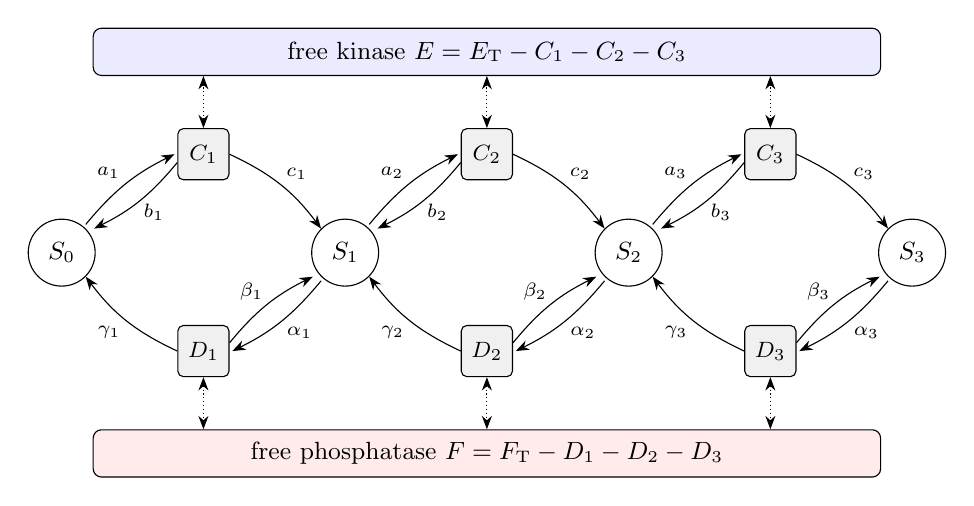
\begin{tikzpicture}[>=Stealth,node distance=20mm,
  sp/.style={circle,draw,minimum size=8.5mm,inner sep=0pt,font=\small},
  cx/.style={rectangle,rounded corners=2pt,draw,minimum size=6.5mm,inner sep=1.5pt,font=\footnotesize,fill=black!6}]
\node[sp] (S0) at (0,0) {$S_0$};
\node[sp] (S1) at (3.6,0) {$S_1$};
\node[sp] (S2) at (7.2,0) {$S_2$};
\node[sp] (S3) at (10.8,0) {$S_3$};
\foreach \i/\a/\b in {1/S0/S1,2/S1/S2,3/S2/S3}{
  \node[cx] (C\i) at ($(\a)!0.5!(\b)+(0,1.25)$) {$C_\i$};
  \node[cx] (D\i) at ($(\a)!0.5!(\b)+(0,-1.25)$) {$D_\i$};
  \draw[->] ([yshift=1.5pt]\a.north east) to[bend left=12] node[above left=-2pt,font=\scriptsize]{$a_\i$} ([xshift=-1pt]C\i.west);
  \draw[->] ([yshift=-3pt]C\i.west) to[bend left=12] node[below right=-3pt,font=\scriptsize]{$b_\i$} ([xshift=3pt]\a.north east);
  \draw[->] (C\i.east) to[bend left=14] node[above right=-2pt,font=\scriptsize]{$c_\i$} (\b.north west);
  \draw[->] ([yshift=-1.5pt]\b.south west) to[bend left=12] node[below right=-2pt,font=\scriptsize]{$\alpha_\i$} ([xshift=1pt]D\i.east);
  \draw[->] ([yshift=3pt]D\i.east) to[bend left=12] node[above left=-3pt,font=\scriptsize]{$\beta_\i$} ([xshift=-3pt]\b.south west);
  \draw[->] (D\i.west) to[bend left=14] node[below left=-2pt,font=\scriptsize]{$\gamma_\i$} (\a.south east);
}
\node[draw,rounded corners=3pt,fill=blue!8,minimum width=100mm,minimum height=6mm,font=\small] (E) at (5.4,2.55) {free kinase $E=\ET-C_1-C_2-C_3$};
\node[draw,rounded corners=3pt,fill=red!8,minimum width=100mm,minimum height=6mm,font=\small] (F) at (5.4,-2.55) {free phosphatase $F=\FT-D_1-D_2-D_3$};
\foreach \i in {1,2,3}{\draw[densely dotted,<->] (C\i.north) -- (C\i.north|-E.south);
                       \draw[densely dotted,<->] (D\i.south) -- (D\i.south|-F.north);}
\end{tikzpicture}
\caption{The three-site sequential distributive cycle $\cN_3$. Each kinase complex $C_i=S_{i-1}E$ and phosphatase complex $D_i=S_iF$ is formed reversibly and resolved irreversibly. All six complexes draw on the two shared free-enzyme pools (dotted); this conservation coupling is the only interaction between sites.}
\label{fig:network}
\end{figure}

\subsection{Results}
All results concern the mass-action system \eqref{eq:network}; stability is always understood within a fixed compatibility class.

\begin{enumerate}[label=(\roman*),leftmargin=*]
\item \textbf{Attracting oscillations for three sites} (Theorem~\ref{thm:main}). There is an explicit family of rate constants, rational in a parameter $r>0$, with an $r$-independent rational positive equilibrium, that undergoes a supercritical Hopf bifurcation at an algebraic value $\rA=1.4332283068\ldots$: a simple pair $\pm\ii\omA$ crosses transversally, the seven complementary eigenvalues are stable, and $l_1<0$. For all small $\rA-r>0$ the system has an orbitally asymptotically stable, strictly positive periodic orbit. Moreover the equilibrium is linearly stable for every $r>\rA$ and has exactly two unstable eigenvalues for every $0<r<\rA$.
\item \textbf{Every $n\ge3$, and the threshold} (Theorems~\ref{thm:alln} and~\ref{thm:threshold}). An explicit site-addition step preserves a nondegenerate Hopf point, its stable complement and the sign of $l_1$; the last point is proved by an exact block computation rather than by an appeal to continuity of centre manifolds. Hence $\cN_n$ admits attracting periodic orbits for every $n\ge3$. Combined with Lemma~\ref{lem:onesite} ($n=1$) and \cite[Theorem~5.8]{Vassena26} ($n=2$), the family $\cN_n$ admits a Hopf bifurcation if and only if $n\ge3$. We also certify concrete supercritical Hopf points for $n=4,5,6$ (Proposition~\ref{prop:explicit}). The step from $n$ to $n+1$ sites is not an instance of the known inheritance theorems for reaction networks \cite{Banaji18,BanajiBorosHofbauer25}; see Remark~\ref{rem:inheritance}.
\item \textbf{An open set of parameters} (Proposition~\ref{prop:robust}). At the three-site Hopf point the derivative of the critical real part with respect to each of the eighteen rate constants and each of the three totals, with the equilibrium free to move, is certified nonzero. Consequently the Hopf set is locally a smooth hypersurface transverse to every coordinate direction of parameter space, and attracting periodic orbits exist on a nonempty open subset of $\R^{21}_{>0}$.
\item \textbf{What static elimination cannot see} (Theorem~\ref{thm:static}, Proposition~\ref{prop:relax}). In equilibrium--flux coordinates the $r$-family keeps fixed the equilibrium, the totals, the productive fluxes and the entire local quasi-steady-state vector field obtained by eliminating all complexes, while its stability changes at $\rA$. No procedure using only those data can predict the oscillation. An admissible change of rate constants that rescales the relaxation of all complexes by a factor $1/\varepsilon$ leaves the same static data fixed, and slowing the complexes destabilizes: $\partial_\varepsilon\Ree\lambda|_{\varepsilon=1}=+0.11207\ldots$ at the Hopf point. The statically eliminated system is Hurwitz stable there.
\item \textbf{Which enzyme pools must be dynamic} (Theorem~\ref{thm:clamp}). If both free enzyme concentrations are held constant, every class has a unique globally attracting equilibrium, for every $n$. If only the free kinase is held constant, Hopf bifurcation still occurs. Dynamic availability of at least one enzyme is thus necessary, and of one enzyme sufficient, for Hopf bifurcation in this architecture.
\item \textbf{A reduction that does work} (Proposition~\ref{prop:reduced}). Eliminating only the fastest complex $C_2$ through its actual nonlinear stationarity equation, and retaining the cubic term that the elimination induces, gives an eight-dimensional system with a supercritical Hopf point whose threshold, frequency and Lyapunov coefficient differ from the true ones by certified small amounts.
\item \textbf{Costs, amplitudes and measurements} (Sections~\ref{sec:resources}--\ref{sec:measure}). On any periodic orbit the time-integrated forward and backward catalytic fluxes agree on every edge separately; the ATP-equivalent turnover per cycle tends to $205.8043\ldots$ at onset while the amplitude vanishes like $\sqrt{\rA-r}$ with certified constants. Numerical continuation (not a proof) follows the attracting branch over the whole interval $0<r<\rA$ to large amplitude, and two points of it, at $r=7/5$ and at the large-amplitude value $r=1$, are certified by a multiple-shooting Newton--Kantorovich argument, including their Floquet multipliers (Theorem~\ref{thm:orbit}). On the stable side the forced response obeys an exact $1/\delta$ resonance law, and a validated finite-time computation shows that a short pulse experiment separates two members of the family that are statically identical but of opposite stability.
\item \textbf{Thermodynamic consistency} (Proposition~\ref{prop:thermo}). Adding chemostatted ATP, ADP and phosphate with reverse catalytic steps obeying local detailed balance gives, for every sufficiently large finite driving affinity, a thermodynamically consistent open network with an attracting periodic orbit.
\end{enumerate}

\subsection{Standard of proof}\label{sec:evidence}
We separate four kinds of evidence and label statements accordingly where it matters.
\begin{description}[leftmargin=2.2em,labelwidth=1.4em,labelsep=0.4em,itemsep=1pt]
\item[\evC] A conventional mathematical proof, using standard theorems (Hopf bifurcation, implicit function theorem, Perron--Frobenius, Routh--Hurwitz).
\item[\evI] A computation in exact rational arithmetic, or in interval arithmetic with outward rounding (rational intervals throughout, binary64 intervals in Theorem~\ref{thm:orbit}), whose inputs are the literal reaction network and whose acceptance conditions are strict inequalities between rational numbers. Floating-point numbers only propose candidates.
\item[\evK] A theorem compiled in Lean~4 with Mathlib.
\item[\evN] Floating-point numerics, used for illustration and discovery only.
\end{description}
The main theorems are \evC+\evI: the analytic step is the classical Hopf theorem \cite{Kuznetsov23,HassardKazarinoffWan81,MarsdenMcCracken76}, and its hypotheses are verified by \evI{} certificates (Section~\ref{sec:cert} and Appendix~\ref{app:cert}). The only \evK{} result is the existence theorem for the earlier subcritical witness (Theorem~\ref{thm:lean}); we do not claim a formal proof of attraction. The script \texttt{check\_paper.py} distributed with the paper rebuilds the network from its reaction list and replays every certified number printed below; it was written independently of the programs used to discover the witnesses, and the two implementations agree.

\subsection{Organisation}
Section~\ref{sec:model} sets up equilibrium--flux coordinates and the pool--complex chart. Section~\ref{sec:hopf} proves the three-site theorem. Section~\ref{sec:alln} treats all $n\ge3$, the threshold and parametric robustness. Section~\ref{sec:mechanism} analyses the mechanism: static invariance, relaxation and clamps. Section~\ref{sec:reduction} gives the selective reduction. Sections~\ref{sec:resources}--\ref{sec:measure} cover finite amplitude, resources and dynamic measurements, Section~\ref{sec:thermo} the driven reversible realization, and Section~\ref{sec:discussion} limitations and open problems.

\section{Equilibrium--flux coordinates and the pool--complex chart}\label{sec:model}

\subsection{The mass-action system}
Order the species as $x=(S_0,\dots,S_n,E,F,C_1,\dots,C_n,D_1,\dots,D_n)\in\R^{3n+3}_{\ge0}$. We index the $2n$ enzymatic \emph{arms} by $j=1,\dots,2n$: arm $j\le n$ is the kinase arm through $z_j=C_j$ and arm $j=n+i$ is the phosphatase arm through $z_{n+i}=D_i$. Arm $j$ has an \emph{input level} $\ell_j$, the phosphorylation level of the substrate it binds, and an enzyme $e_j$:
\[
 \ell_j=j-1,\quad e_j=E\quad(j\le n);\qquad \ell_{n+i}=i,\quad e_{n+i}=F\quad(1\le i\le n).
\]
Writing $k_j$ for the binding constant ($a_i$ or $\alpha_i$), $k_j^{-}$ for the dissociation constant ($b_i$ or $\beta_i$) and $k_j^{\mathrm c}$ for the catalytic constant ($c_i$ or $\gamma_i$), the complexes obey
\begin{equation}\label{eq:complex-ode}
 \dot z_j=k_j\,S_{\ell_j}\,e_j-(k_j^{-}+k_j^{\mathrm c})\,z_j ,\qquad j=1,\dots,2n,
\end{equation}
and the remaining equations follow from \eqref{eq:network}; for example $\dot S_i=c_iC_i-a_{i+1}S_iE+b_{i+1}C_{i+1}-\alpha_iS_iF+\beta_iD_i+\gamma_{i+1}D_{i+1}$ for $1\le i\le n-1$. The vector field is quadratic. The stoichiometric matrix has rank $3n$, the three totals \eqref{eq:totals} are conserved, and the nonnegative orthant is forward invariant. For positive totals we write $\cP=\cP(\ET,\FT,\ST)$ for the set of nonnegative states with those totals; it is compact and convex, so all solutions exist for all time and are bounded.

\subsection{All positive equilibria, parametrized}
The search for a Hopf point in eighteen rate constants and three totals is ill-conditioned; the following coordinates turn it into a search over quantities with direct meaning, and keep the equilibrium exactly rational.

\begin{lemma}[Equilibrium--flux coordinates]\label{lem:coords}
Let $x^*\in\R^{3n+3}_{>0}$. The point $x^*$ is an equilibrium of $\cN_n$ with positive rate constants if and only if there are numbers $q_i>0$ and $\rho_i,\sigma_i>0$ $(1\le i\le n)$ such that
\begin{equation}\label{eq:rates}
\begin{aligned}
 a_i&=\frac{(1+\rho_i)\,q_i}{S_{i-1}^*E^*},& b_i&=\frac{\rho_i\,q_i}{C_i^*},& c_i&=\frac{q_i}{C_i^*},\\
 \alpha_i&=\frac{(1+\sigma_i)\,q_i}{S_i^*F^*},& \beta_i&=\frac{\sigma_i\,q_i}{D_i^*},& \gamma_i&=\frac{q_i}{D_i^*}.
\end{aligned}
\end{equation}
The map $(x^*,q,\rho,\sigma)\mapsto(\text{rate constants},\,x^*)$ is a bijection from $\R^{3n+3}_{>0}\times\R^{3n}_{>0}$ onto the set of pairs (rate constants, positive equilibrium).
\end{lemma}
\begin{proof}
If \eqref{eq:rates} holds, then $a_iS_{i-1}^*E^*=(1+\rho_i)q_i=(b_i+c_i)C_i^*$, so each $\dot C_i$ vanishes, and likewise each $\dot D_i$. The two catalytic fluxes on edge $i$ are $c_iC_i^*=q_i=\gamma_iD_i^*$; inserting the complex balances into the equation for $\dot S_i$ leaves $q_i-q_{i+1}-q_i+q_{i+1}=0$ (with the obvious modification at $i=0,n$), and $\dot E=-\sum\dot C_i=0$, $\dot F=-\sum\dot D_i=0$. Conversely, at a positive equilibrium put $q_i=c_iC_i^*$, $\rho_i=b_i/c_i$, $q_i'=\gamma_iD_i^*$, $\sigma_i=\beta_i/\gamma_i$. Stationarity of $C_i$ and $D_i$ gives the formulas for $a_i$ and $\alpha_i$ with $q_i'$ in place of $q_i$ on the phosphatase arm, and stationarity of the pool $u_i$ of \eqref{eq:pools} below gives $q_i=q_i'$. The inverse map is explicit, so the correspondence is bijective.
\end{proof}
We call $q_i$ the \emph{productive flux} on edge $i$ and $\rho_i=b_i/c_i$, $\sigma_i=\beta_i/\gamma_i$ the \emph{reverse ratios}. The gross binding flux of arm $j$ at equilibrium is
\begin{equation}\label{eq:v}
 v_j=(1+\rho_j)q_j\quad(j\le n),\qquad v_{n+i}=(1+\sigma_i)q_i .
\end{equation}

\subsection{Cumulative pools and the chart}
Binding and dissociation do not change the phosphorylation level of the substrate molecule involved, if a complex is counted at its input level. Define the \emph{cumulative pools}
\begin{equation}\label{eq:pools}
 u_i=\sum_{l\ge i}S_l+\sum_{j:\ \ell_j\ge i}z_j
    =\sum_{l=i}^{n}S_l+\sum_{l=i+1}^{n}C_l+\sum_{l=i}^{n}D_l,\qquad i=1,\dots,n ,
\end{equation}
the amount of substrate, free or bound, at level at least $i$. Only the two catalytic steps on edge $i$ move substrate across the boundary between levels $i-1$ and $i$, so
\begin{equation}\label{eq:pooldot}
 \dot u_i=c_iC_i-\gamma_iD_i ,\qquad\text{that is}\qquad \dot u=Lz,\quad L=\bigl[\diag(c_i)\,,\ -\diag(\gamma_i)\bigr]\in\R^{n\times2n}.
\end{equation}
This identity is exact and linear. On a class $\cP$ the pair $(u,z)\in\R^n\times\R^{2n}$ determines the state: with $u_0=\ST$ and $u_{n+1}=0$,
\begin{equation}\label{eq:lift}
 S_l=u_l-u_{l+1}-\sum_{j:\ \ell_j=l}z_j,\qquad E=\ET-\sum_{j\le n}z_j,\qquad F=\FT-\sum_{j>n}z_j .
\end{equation}
Thus $(u,z)$ is an affine chart of $\cP$. In matrix form, for deviations from an equilibrium, $\delta S=T\delta u-H_S\delta z$ and $\delta(E,F)^{\T}=-H_E\delta z$, where $T\in\R^{(n+1)\times n}$ has $T_{l,l}=1$, $T_{l,l+1}=-1$ (rows $l=0,\dots,n$, columns $1,\dots,n$), and $H_S\in\R^{(n+1)\times2n}$, $H_E\in\R^{2\times2n}$ are the incidence matrices $(H_S)_{l,j}=[\ell_j=l]$, $(H_E)_{e,j}=[e_j=e]$.

In this chart \eqref{eq:complex-ode} takes a form in which the role of each parameter is transparent: using $k_jS^*_{\ell_j}e_j^*=v_j=(k_j^-+k_j^{\mathrm c})z_j^*$,
\begin{equation}\label{eq:chartfield}
 \dot u=Lz,\qquad
 \dot z_j=v_j\left[\frac{S_{\ell_j}(u,z)\,e_j(z)}{S_{\ell_j}^*\,e_j^*}-\frac{z_j}{z_j^*}\right],\quad j=1,\dots,2n ,
\end{equation}
with $S_{\ell_j}(u,z)$ and $e_j(z)$ the affine functions \eqref{eq:lift}.

\begin{lemma}[Block structure]\label{lem:blocks}
Let $y=(\delta u,\delta z)$ denote deviations from a positive equilibrium. The field \eqref{eq:chartfield} is $\dot y=Jy+\tfrac12B(y,y)$ with
\begin{equation}\label{eq:J}
 J=\begin{pmatrix}0&L\\ M&-A\end{pmatrix},\qquad A=VG,\quad M=VN,\quad V=\diag(v_1,\dots,v_{2n}),
\end{equation}
\begin{equation}\label{eq:GN}
 G=\diag(1/z^*)+H_S^{\T}\diag(1/S^*)H_S+H_E^{\T}\diag(1/E^*,1/F^*)H_E,\qquad N=H_S^{\T}\diag(1/S^*)\,T ,
\end{equation}
and the only nonzero components of the symmetric bilinear map $B$ are
\begin{equation}\label{eq:B}
 B_{n+j}(h,k)=k_j\bigl[\delta S_{\ell_j}(h)\,\delta e_j(k)+\delta S_{\ell_j}(k)\,\delta e_j(h)\bigr],\qquad k_j=\frac{v_j}{S_{\ell_j}^*e_j^*}.
\end{equation}
The matrix $G$ is symmetric positive definite and does not depend on the reverse ratios. Consequently $A$ is similar to the symmetric positive definite matrix $V^{1/2}GV^{1/2}$: at frozen pools the complexes relax with real, strictly positive rates.
\end{lemma}
\begin{proof}
Differentiate \eqref{eq:chartfield}: $\delta\dot z_j=v_j[\delta S_{\ell_j}/S^*_{\ell_j}+\delta e_j/e_j^*-\delta z_j/z_j^*]$ and insert $\delta S=T\delta u-H_S\delta z$, $\delta e=-H_E\delta z$. For $w\ne0$, $w^{\T}Gw=\sum_jw_j^2/z_j^*+\sum_l(H_Sw)_l^2/S_l^*+\sum_e(H_Ew)_e^2/e^*>0$. The second-order part of the product $S_{\ell_j}e_j$ gives \eqref{eq:B}.
\end{proof}
The zero block in \eqref{eq:J} records that pools are moved only by complexes; the term $H_E^{\T}\diag(1/E^*,1/F^*)H_E$ in $G$ is the \emph{enzyme-availability coupling}: every complex of an enzyme lowers the binding flux of all complexes of the same enzyme. It is the only place where the sharing of the enzymes enters the linearization, and it disappears for an enzyme whose free concentration is held fixed (Section~\ref{sec:clamp}).

\subsection{Two explicit three-site families}\label{sec:witnesses}
For $n=3$ we use two one-parameter families. In both, all reverse ratios equal $1/100$ except $\sigma_1=r>0$, which is the bifurcation parameter; by \eqref{eq:rates} only $\alpha_1$ and $\beta_1$ depend on $r$, and the equilibrium, the totals and the productive fluxes do not.

\paragraph{Witness $\WA$ (attracting).}
\begin{equation}\label{eq:witnessA}
\begin{aligned}
 x^*_{\WA}&=\Bigl(\underbrace{2,\ 12,\ \tfrac15,\ \tfrac25}_{S_0,\dots,S_3},\ \underbrace{\tfrac{23}{10},\ \tfrac25}_{E,\ F},\ \underbrace{\tfrac{23}{50},\ \tfrac3{10},\ \tfrac{17}{10}}_{C_1,C_2,C_3},\ \underbrace{23,\ \tfrac9{50},\ 4}_{D_1,D_2,D_3}\Bigr),\\
 q&=\bigl(\tfrac1{10},\tfrac{32}5,\tfrac65\bigr),\qquad \rho=\bigl(\tfrac1{100},\tfrac1{100},\tfrac1{100}\bigr),\qquad \sigma=\bigl(r,\tfrac1{100},\tfrac1{100}\bigr),
\end{aligned}
\end{equation}
with totals $(\ET,\FT,\ST)=(119/25,\;1379/50,\;1106/25)=(4.76,\;27.58,\;44.24)$. The rate constants are listed in Table~\ref{tab:ratesA}.

\paragraph{Witness $\WH$ (subcritical, formally verified existence).}
\begin{equation}\label{eq:witnessH}
 x^*_{\WH}=\bigl(30,13,\tfrac{19}{100},\tfrac9{100},\tfrac{33}{10},1,\tfrac{13}{25},\tfrac7{250},\tfrac{39}{50},\tfrac{93}{10},\tfrac3{20},\tfrac52\bigr),\qquad q=\bigl(\tfrac1{10},\tfrac{39}5,1\bigr),
\end{equation}
with the same reverse ratios and totals $(1157/250,\;259/20,\;28279/500)$. Its rate constants are, in the order of Table~\ref{tab:ratesA}: $(101/99000,\,1/520,\,5/26)$, $(101/550,\,39/14,\,1950/7)$, $(1010/627,\,1/78,\,50/39)$ for the kinase arms and $((1+r)/130,\,r/93,\,1/93)$, $(3939/95,\,13/25,\,52)$, $(101/9,\,1/250,\,2/5)$ for the phosphatase arms. This is the first Hopf point we found in $\cN_3$; its bifurcation is subcritical (Section~\ref{sec:lean}).

\begin{table}[htbp]
\centering
\begin{tabular}{c@{\qquad}ccc@{\qquad}ccc}
\toprule
Site $i$ & $a_i$ & $b_i$ & $c_i$ & $\alpha_i$ & $\beta_i$ & $\gamma_i$\\
\midrule
1 & $101/4600$ & $1/460$ & $5/23$ & $(1+r)/48$ & $r/230$ & $1/230$\\
2 & $404/1725$ & $16/75$ & $64/3$ & $404/5$ & $16/45$ & $320/9$\\
3 & $303/115$ & $3/425$ & $12/17$ & $303/40$ & $3/1000$ & $3/10$\\
\bottomrule
\end{tabular}
\caption{The eighteen rate constants of witness $\WA$, from \eqref{eq:rates} and \eqref{eq:witnessA}. All are positive rationals for rational $r>0$; the critical value $\rA$ itself is algebraic. The ratio of largest to smallest catalytic constant is $73600/9\approx8178$ and of binding constants $3680$ (near $r=\rA$); binding and first-order constants carry different units and are not compared.}
\label{tab:ratesA}
\end{table}

\section{A supercritical Hopf bifurcation for three sites}\label{sec:hopf}

\begin{theorem}[Attracting oscillations in $\cN_3$; \evC+\evI]\label{thm:main}
Consider $\cN_3$ with the rate constants of Table~\ref{tab:ratesA}, on the compatibility class $(\ET,\FT,\ST)=(119/25,1379/50,1106/25)$, in which $x^*_{\WA}$ is an equilibrium for every $r>0$. There are algebraic numbers $\rA,\omA$ with
\[
 1.43322830681119<\rA<1.43322830681120,\quad 0.23508019956219<\omA<0.23508019956220
\]
such that:
\begin{enumerate}[label=\textup{(\alph*)}]
\item at $r=\rA$ the reduced $9\times9$ Jacobian $J(r)$ has the simple eigenvalues $\pm\ii\omA$ and seven eigenvalues with negative real part;
\item the eigenvalue branch $\lambda(r)$ through $\ii\omA$ satisfies $-0.05131591007519<\Ree\lambda'(\rA)<-0.05131591007517$;
\item the first Lyapunov coefficient satisfies $-0.08915942680579<l_1<-0.08915942680577$.
\end{enumerate}
Consequently the family undergoes a supercritical Hopf bifurcation at $\rA$: there is $\mu_0>0$ such that for every $r\in(\rA-\mu_0,\rA)$ the system has a nonconstant periodic orbit in the class, lying in the open positive orthant, which is orbitally asymptotically stable within the class; its period tends to $2\pi/\omA=26.7278372\ldots$ and its diameter to zero as $r\uparrow\rA$. Moreover $x^*_{\WA}$ is linearly stable for every $r>\rA$ and has exactly two eigenvalues in the open right half-plane for every $0<r<\rA$.
\end{theorem}

The normalizations behind \textup{(c)} are $q_{D_3}=1$ for the critical right eigenvector and $p^{\T}q=1$ for the left one (Section~\ref{sec:cert}); the sign of $l_1$ does not depend on them. The theorem is local in $r$: it gives no value of $\mu_0$. Section~\ref{sec:resources} shows numerically that the attracting branch in fact persists for all $0<r<\rA$.

\subsection{The certificate}\label{sec:cert}
We describe the computation for a general family in which one reverse ratio varies; it is used unchanged for every Hopf point in this paper. Let $d$ be the dimension of the chart ($d=9$ for $\cN_3$).

\paragraph{Step 1: an affine characteristic polynomial.} By \eqref{eq:J}--\eqref{eq:GN} the parameter $r=\sigma_1$ enters $J$ only through $v_{n+1}=(1+r)q_1$, which multiplies the single row of $J$ belonging to $D_1$. The determinant is linear in each row, so
\begin{equation}\label{eq:p}
 p(s,r)=\det\bigl(sI-J(r)\bigr)=p_0(s)+r\,p_1(s),\qquad p_0,p_1\in\mathbb Q[s],
\end{equation}
with $p_0$ monic of degree $d$ and $\deg p_1<d$. Both polynomials are computed exactly from the reaction list, and the identity \eqref{eq:p} is checked at a third value of $r$.

\paragraph{Step 2: the frequency eliminant.} Split $p_k(\ii\sqrt t)=E_k(t)+\ii\sqrt t\,O_k(t)$ with $E_k,O_k\in\mathbb Q[t]$. A pair $\pm\ii\sqrt t$, $t>0$, is a root of $p(\cdot,r)$ if and only if $E_0+rE_1=0=O_0+rO_1$ at $t$, which implies
\begin{equation}\label{eq:Phi}
 \Phi(t):=O_0(t)E_1(t)-E_0(t)O_1(t)=0 .
\end{equation}
A Sturm sequence shows that $\Phi$ has exactly one root $t_{\mathrm A}$ in $[0,\infty)$, that it is simple, and isolates it in a rational interval of width below $10^{-55}$; for witness $\WA$, $0.0552627002262007<t_{\mathrm A}<0.0552627002262009$. On that interval $E_1^2+tO_1^2$ is bounded away from zero, and we set
\begin{equation}\label{eq:r}
 \omA=\sqrt{t_{\mathrm A}},\qquad \rA=-\frac{E_0E_1+t\,O_0O_1}{E_1^2+t\,O_1^2}\Big|_{t=t_{\mathrm A}} .
\end{equation}
Then $E_0+\rA E_1=-t\,O_1\Phi/(E_1^2+tO_1^2)=0$ and $O_0+\rA O_1=E_1\Phi/(E_1^2+tO_1^2)=0$ at $t_{\mathrm A}$, so $\pm\ii\omA$ are roots of $p(\cdot,\rA)$ exactly; conversely \eqref{eq:r} is the only value of $r$ with a purely imaginary pair. The interval for $\rA$ is strictly positive.

\paragraph{Step 3: the other eigenvalues.} Interval synthetic division of $p(\cdot,\rA)$ by $s^2+t_{\mathrm A}$ encloses the coefficients of the exact quotient $g$, of degree $d-2$. Every entry of the first column of the Routh array of $g$ is an interval with positive lower endpoint; for $\WA$ these lower endpoints exceed
\[
 1,\quad 123,\quad 4107,\quad 57834,\quad 328922,\quad 598584,\quad 160490,\quad 6202 .
\]
By the Routh--Hurwitz criterion all roots of $g$ lie in the open left half-plane. In particular $\pm\ii\omA$ are simple, and $J$ and $2\ii\omA I-J$ are invertible.

\paragraph{Step 4: transversality.} Implicit differentiation of \eqref{eq:p} gives $\lambda'(\rA)=-p_1(\ii\omA)/\partial_sp(\ii\omA,\rA)$; the denominator is enclosed away from zero and the real part of the quotient is enclosed as in \textup{(b)}.

\paragraph{Step 5: the first Lyapunov coefficient.} Let $Jq=\ii\omA q$ with $q_{D_3}=1$ and $p^{\T}J=\ii\omA p^{\T}$ with $p^{\T}q=1$ (a bilinear pairing; $p$ is the complex conjugate of the adjoint eigenvector in the Hermitian convention). Since the field is quadratic, with $B$ as in \eqref{eq:B}, the first Lyapunov coefficient in the convention of \cite[Sections~3.5 and~5.4]{Kuznetsov23} is
\begin{equation}\label{eq:l1}
 l_1=\frac1{2\omA}\Ree\, p^{\T}\Bigl[-2B\bigl(q,J^{-1}B(q,\bar q)\bigr)+B\bigl(\bar q,(2\ii\omA I-J)^{-1}B(q,q)\bigr)\Bigr];
\end{equation}
a cubic term $p^{\T}C(q,q,\bar q)$ is added inside the bracket when the field has one (Section~\ref{sec:reduction}). The eigenvectors are obtained by interval Gaussian elimination on the $(d-1)\times(d-1)$ system that remains after fixing the normalized coordinate; every pivot is an interval that excludes zero, which also proves that this minor is invertible for every matrix in the interval family, and the two resolvent solves are enclosed in the same way. With these normalizations the sign of $l_1$ equals the sign of the cubic coefficient of the radial normal form, which is $\omA l_1\in(-0.0209597,-0.0209596)$ in the time unit of the model.

\paragraph{Arithmetic.} Real intervals have rational endpoints. After each operation the endpoints are rounded outward to the grid $2^{-160}\mathbb Z$; products take the extreme endpoint products, a quotient is refused unless the divisor interval excludes zero, and square roots are bounded by integer square roots. Complex intervals are pairs of real ones. All acceptance conditions are inequalities between rational numbers, and the widths of the final enclosures are below $10^{-33}$; the windows printed in this paper are coarser and contain them. See Appendix~\ref{app:cert}.

\begin{proof}[Proof of Theorem~\ref{thm:main}]
Statements (a)--(c) are the output of Steps~1--5 for the family \eqref{eq:witnessA}. The chart field \eqref{eq:chartfield} is polynomial in $y$ and in $r$, and $y=0$ is an equilibrium for all $r$. By (a) the linearization at $r=\rA$ has a simple pair $\pm\ii\omA$ and no other spectrum on the imaginary axis; by (b) the pair crosses transversally; by (c) the bifurcation is nondegenerate with $l_1<0$. The Hopf bifurcation theorem, in the form obtained by reduction to a parameter-dependent two-dimensional centre manifold \cite[Sections~3.5 and~5.4]{Kuznetsov23}, see also \cite{HassardKazarinoffWan81,MarsdenMcCracken76}, yields a unique small limit cycle on the side where the equilibrium is unstable, here $r<\rA$ because $\Ree\lambda'(\rA)<0$. On the centre manifold the cycle is attracting because $l_1<0$; the centre manifold is itself exponentially attracting because the other seven eigenvalues are stable. Hence the cycle is orbitally asymptotically stable in the chart, that is, within $\cP$; with $a:=-\Ree\lambda'(\rA)$ and $\mu:=\rA-r$ the radial normal form is
\begin{equation}\label{eq:radial}
 \dot\varrho=a\mu\,\varrho+\omA l_1\,\varrho^3+O(\varrho^5+\mu^2\varrho) .
\end{equation}
The chart \eqref{eq:lift} preserves the totals, and $x^*_{\WA}$ has positive coordinates, so sufficiently small cycles are positive. The period tends to $2\pi/\omA$.

For the last assertion, an eigenvalue can reach the imaginary axis at $r_0>0$ only if $p(0,r_0)=0$ or $p(\ii\sqrt t,r_0)=0$ for some $t>0$. The first is impossible because $p_0(0)>0$ and $p_1(0)\ge0$ (exact rationals). The second forces $\Phi(t)=0$, hence $t=t_{\mathrm A}$ and then $r_0=\rA$ by Step~2. The roots of the monic polynomial $p(\cdot,r)$ depend continuously on $r$ and stay bounded on compact parameter sets, so the number of roots in the open right half-plane is constant on $(0,\rA)$ and on $(\rA,\infty)$; by (a) and (b) it is $2$ just below $\rA$ and $0$ just above.
\end{proof}

\begin{remark}[The critical mode]\label{rem:mode}
With $q_{D_3}=1$ the critical eigenvector is, to four digits (\evN),
\[
\begin{array}{c|ccccccccc}
 & u_1&u_2&u_3&C_1&C_2&C_3&D_1&D_2&D_3\\\hline
|q| & 0.035&1.744&1.278&0.049&0.082&0.508&0.919&0.055&1\\
\arg q & 131^\circ&28^\circ&17^\circ&-159^\circ&-124^\circ&53^\circ&158^\circ&-113^\circ&0^\circ
\end{array}
\]
The oscillation lives in the upper pools $u_2,u_3$ and in the complexes $D_1$, $D_3$, $C_3$. At the equilibrium $D_1=S_1F$ holds $23/27.58\approx83\%$ of the phosphatase, the three phosphatase complexes together $1359/1379\approx98.5\%$, and $D_1$ is resolved by the slowest catalytic step ($\gamma_1=1/230$). Its component is almost in antiphase with that of $D_3$ ($158^\circ$): phosphatase is handed back and forth between the low and the high end of the chain. We refrain from turning these phases into a scalar delay-line argument; Section~\ref{sec:mechanism} gives the statements about mechanism that we can prove.
\end{remark}

\subsection{The subcritical witness and its formal verification}\label{sec:lean}
The same certificate applied to the family \eqref{eq:witnessH} gives
\begin{equation}\label{eq:Hdata}
\begin{gathered}
 0.26553704252<\rH<0.26553704254,\qquad 0.18038559401<\omH<0.18038559403,\\
 -0.04649665728<\Ree\lambda'(\rH)<-0.04649665726,\qquad 0.66961007953<l_1<0.66961007956,
\end{gathered}
\end{equation}
with a Hurwitz complementary factor (the Routh column is bounded below by $1$, $406$, $35862$, $1085458$, $10924589$, $24494015$, $5131445$, $15020$). Thus $\WH$ has a \emph{subcritical} Hopf bifurcation: small periodic orbits exist for $r>\rH$, where the equilibrium is stable, and they are orbitally unstable. As for $\WA$, the equilibrium is stable for all $r>\rH$ and has two unstable eigenvalues for $0<r<\rH$.

For this witness the existence of periodic orbits has been verified in Lean~4, independently of the interval certificate and without importing a Hopf theorem.

\begin{theorem}[Formally verified existence at $\WH$; \evK]\label{thm:lean}
There exist $r_0,w>0$ and a smooth local eigenvalue branch $g(r)$ of the reduced Jacobian of the family \eqref{eq:witnessH} with $g(r_0)=\ii w$ and $(\Ree g)'(r_0)<0$. For every $\varepsilon>0$ there are $r,T>0$ with $|r-r_0|<\varepsilon$, $|T-2\pi/w|<\varepsilon$, and a nonconstant $T$-periodic solution $\varphi:\R\to\R^{12}$ of the mass-action equations of $\cN_3$ with the rate constants of $\WH$ at parameter $r$, such that all eighteen rate constants are positive, $\varphi_i(t)>0$ and $\|\varphi(t)-x^*_{\WH}\|_\infty<\varepsilon$ for all $t$, and the three totals of $\varphi(t)$ equal those of $x^*_{\WH}$.
\end{theorem}
The Lean statement is \lean{ThreeSitePhosphorylation.three_site_hopf_capacity}; it has no hypotheses, and its axioms are the three standard ones of Mathlib's classical logic. The proof constructs the critical frequency from rational polynomial inequalities and the intermediate value theorem, locates the seven real complementary eigenvalues in disjoint rational intervals, and obtains the periodic orbits from a rescaled shooting problem $u'=T\{J(r)u+a\,Q(r,u)\}$ solved by the implicit function theorem at amplitude $a=0$; invertibility of the $11\times11$ derivative is the Fredholm-type argument that the resonant coefficient $T\lambda'(r_0)\delta r+\ii w\,\delta T$ must vanish. The theorem asserts neither a least period nor stability; the sign of $l_1$ in \eqref{eq:Hdata}, and everything about witness $\WA$, is \evC+\evI.

\begin{remark}[From $\WH$ to $\WA$]
Coordinate-wise continuation of Hopf points from $\WH$ in the variables of Lemma~\ref{lem:coords} never changed the sign of $l_1$ (96 continuations), but indicated that increasing $S_3^*$ lowers it. A gradient descent on $l_1$ in the logarithms of the equilibrium and flux coordinates, corrected at each step back onto the Hopf surface, reached $l_1<0$ with a stable complement after 65 evaluations. Rounding to small rationals preserved the signs; raising the occupancy $C_2^*$ and lowering $S_0^*$ then reduced the spread of the rate constants and gave \eqref{eq:witnessA}. Along a log-affine path between the two witnesses, floating-point continuation shows $l_1$ changing sign once, with stable complement and negative crossing throughout (\evN). This suggests a Bautin (generalized Hopf) point, and hence parameter regions where a stable equilibrium coexists with a stable periodic orbit; we have not certified it.
\end{remark}

\section{Every \texorpdfstring{$n\ge3$}{n >= 3}, the threshold, and an open set of parameters}\label{sec:alln}

\subsection{Adding a site}
\begin{theorem}[Site addition; \evC]\label{thm:alln}
Let $n\ge1$ and let $\cN_n$ carry a smooth one-parameter family of positive rate constants with an $r$-independent positive equilibrium $x^*$. Suppose that at $r=r_0$ the reduced Jacobian $J_n(r_0)$ has a simple pair $\pm\ii\omega_0$, $\omega_0>0$, all other eigenvalues in the open left half-plane, $\Ree\lambda'(r_0)\ne0$ and $l_1\ne0$. For $\epsilon>0$ keep all rate constants of $\cN_n$ and give the new site of $\cN_{n+1}$ the rate constants
\begin{equation}\label{eq:newrates}
 (a_{n+1},b_{n+1},c_{n+1})=\Bigl(\frac{2\epsilon}{S_n^*E^*},\,1,\,1\Bigr),\qquad
 (\alpha_{n+1},\beta_{n+1},\gamma_{n+1})=\Bigl(\frac1{F^*},\,1,\,1\Bigr).
\end{equation}
Then $x^*$, completed by $C_{n+1}^*=D_{n+1}^*=\epsilon$ and $S_{n+1}^*=2\epsilon$, is a positive equilibrium of $\cN_{n+1}$ for every $r$, with totals $(\ET+\epsilon,\FT+\epsilon,\ST+4\epsilon)$; in the coordinates of Lemma~\ref{lem:coords}, $q_{n+1}=\epsilon$ and $\rho_{n+1}=\sigma_{n+1}=1$. For every sufficiently small $\epsilon>0$ there is $r(\epsilon)$, with $r(\epsilon)\to r_0$, at which the $(n+1)$-site family has a simple pair of purely imaginary eigenvalues, all other eigenvalues in the open left half-plane, a transversal crossing in the same direction, and a first Lyapunov coefficient of the same sign as $l_1$.
\end{theorem}
\begin{proof}
\emph{Equilibrium.} Both new binding fluxes equal $2\epsilon$, both new dissociation fluxes and both new catalytic fluxes equal $\epsilon$. The new site therefore removes $2\epsilon-\epsilon-\epsilon=0$ from $S_n$, from $E$ and from $F$, all old balances are unchanged, and the new complexes and $S_{n+1}$ are stationary.

\emph{A chart that isolates the new site.} On the new class use the coordinates $(y,w)$, where $w=(C_{n+1},S_{n+1},D_{n+1})-\epsilon(1,2,1)$ and $y=(\delta\tilde u,\delta z)$ with $\tilde u_i$ $(i\le n)$ the old pools \eqref{eq:pools}, which do not count the three new species. The old free species are recovered by \eqref{eq:lift} with the new totals diminished by the new inventories, e.g.\ $E=\ET+\epsilon-\sum_{i\le n}C_i-C_{n+1}$. This is an affine chart of the new class, affinely equivalent to its pool--complex chart, and the vector field in it is a polynomial in $(y,w)$ whose coefficients are polynomials in $\epsilon$ and smooth in $r$; it is defined for $\epsilon$ in a neighbourhood of $0$, including $\epsilon\le0$ where it has no chemical meaning. The new equations are
\begin{equation}\label{eq:newsite}
 \dot C_{n+1}=a_{n+1}S_nE-2C_{n+1},\qquad \dot S_{n+1}=C_{n+1}-\frac{F}{F^*}S_{n+1}+D_{n+1},\qquad \dot D_{n+1}=\frac{F}{F^*}S_{n+1}-2D_{n+1},
\end{equation}
and every old pool acquires the extra term $-a_{n+1}S_nE+C_{n+1}+D_{n+1}$.

\emph{The limit $\epsilon=0$.} Then $a_{n+1}=0$ and the base point has $C_{n+1}=S_{n+1}=D_{n+1}=0$. Every term of \eqref{eq:newsite} contains a factor $w_k$, so $\{w=0\}$ is invariant, and on it the field is exactly the $n$-site field $\dot y=J_ny+\tfrac12B_n(y,y)$. Hence the system has the form
\begin{equation}\label{eq:triangular}
 \dot y=J_n(r)y+U(r)w+\tfrac12B_n(y,y)+R_1(y,w),\qquad \dot w=Kw+R_2(y,w),\qquad
 K=\begin{pmatrix}-2&0&0\\1&-1&1\\0&1&-2\end{pmatrix},
\end{equation}
where $R_1,R_2$ are bilinear and every monomial of them contains a component of $w$. The Jacobian $\tilde J=\bigl(\begin{smallmatrix}J_n&U\\0&K\end{smallmatrix}\bigr)$ is block triangular and $\det(sI-K)=(s+2)(s^2+3s+1)$ has the roots $-2,(-3\pm\sqrt5)/2$. Thus at $(\epsilon,r)=(0,r_0)$ the pair $\pm\ii\omega_0$ is simple and all other eigenvalues are stable.

\emph{The Lyapunov coefficient at $\epsilon=0$.} The critical right eigenvector is $\tilde q=(q,0)$. The left eigenvector is $\tilde p=(p,p_w)$ with $p_w^{\T}=p^{\T}U(\ii\omega_0-K)^{-1}$, and $\tilde p^{\T}\tilde q=p^{\T}q=1$. Write $\tilde B$ for the quadratic part of \eqref{eq:triangular}. Because every monomial of $R_1,R_2$ contains a component of $w$, $\tilde B\bigl((y_1,0),(y_2,0)\bigr)=\bigl(B_n(y_1,y_2),0\bigr)$. Because $\tilde J$ is block triangular, $\tilde J^{-1}(v,0)=(J_n^{-1}v,0)$ and $(2\ii\omega_0-\tilde J)^{-1}(v,0)=((2\ii\omega_0-J_n)^{-1}v,0)$. Inserting these into \eqref{eq:l1} shows that every vector occurring there has the form $(\cdot,0)$ and that $\tilde p$ is only ever paired with such vectors, so
\[
 l_1^{(n+1)}\big|_{\epsilon=0}=l_1^{(n)} ,\qquad\text{and likewise}\qquad \tilde p^{\T}(\partial_r\tilde J)\tilde q=p^{\T}(\partial_rJ_n)q=\lambda'(r_0).
\]

\emph{Small $\epsilon>0$.} The simple eigenvalue $\lambda(\epsilon,r)$ is smooth near $(0,r_0)$, and $\partial_r\Ree\lambda(0,r_0)\ne0$, so the implicit function theorem gives a smooth curve $r(\epsilon)$ with $\Ree\lambda(\epsilon,r(\epsilon))=0$. The other eigenvalues, the normalized eigenvectors, the resolvents in \eqref{eq:l1} and hence $l_1$ depend continuously on $\epsilon$ along this curve. Stability of the complement, the sign of the crossing and the sign of $l_1$ therefore persist for small $\epsilon$; for $\epsilon>0$ the equilibrium and all rate constants are positive.
\end{proof}

The extended family again has an $r$-independent equilibrium, with unchanged $E^*$ and $F^*$, so the step can be iterated.

\begin{corollary}[Attracting oscillations for every $n\ge3$; \evC+\evI]\label{cor:alln}
For every $n\ge3$ there are positive rate constants and totals for which $\cN_n$ has a supercritical Hopf bifurcation with stable complement, and hence orbitally asymptotically stable, strictly positive periodic orbits.
\end{corollary}
\begin{proof}
Start from Theorem~\ref{thm:main} and apply Theorem~\ref{thm:alln} $n-3$ times, fixing at each step a sufficiently small positive load $\epsilon$. For the final family apply the Hopf theorem as in the proof of Theorem~\ref{thm:main}, choosing the amplitude small relative to the distance of the (now fixed, positive) equilibrium from the boundary of the orthant.
\end{proof}
The order of quantifiers matters: the loads are fixed first, and no bound on loads, amplitudes or rate constants uniform in $n$ is asserted.

\begin{remark}[Relation to inheritance theorems]\label{rem:inheritance}
Banaji and coauthors have shown that nondegenerate behaviour, including supercritical Hopf bifurcation, is inherited by a network from a subnetwork under six kinds of enlargement \cite{Banaji18,BanajiBorosHofbauer22,Banaji23,BanajiBorosHofbauer25}. The passage from $\cN_n$ to $\cN_{n+1}$ does not appear to be a composition of these: the new species $S_{n+1}$ is produced and consumed only by irreversible steps mediated by two \emph{existing} enzymes, whereas the enlargements that introduce enzymatic mechanisms require new enzymes, and the closest chain of admissible enlargements we found leaves a spurious reaction $S_{n+1}+E\to S_n+E$ that cannot subsequently be removed. Theorem~\ref{thm:alln} is a direct proof tailored to \eqref{eq:network}; its mechanism (a boundary equilibrium of a regular perturbation, an invariant face carrying the old dynamics, and a Hurwitz transverse block) is in the spirit of \cite{BanajiBorosHofbauer25}.
\end{remark}

\begin{proposition}[Explicit witnesses for $n=4,5,6$; \evI]\label{prop:explicit}
Append to witness $\WA$ one, two or three sites by \eqref{eq:newrates}, each with load $\epsilon=1/100$. The certificate of Section~\ref{sec:cert}, with $q_{D_3}=1$, gives for the resulting families of $\cN_4,\cN_5,\cN_6$:
\begin{center}\small
\begin{tabular}{cccccc}
\toprule
$n$ & $(\ET,\FT,\ST)$ & $r_{\rm Hopf}$ & $\omega$ & $\Ree\lambda'$ & $l_1$\\
\midrule
3 & $(4.76,\ 27.58,\ 44.24)$ & $1.433228306811$ & $0.235080199562$ & $-0.0513159101$ & $-0.0891594268$\\
4 & $(4.77,\ 27.59,\ 44.28)$ & $1.367207896571$ & $0.228851319852$ & $-0.0508490424$ & $-0.1071919621$\\
5 & $(4.78,\ 27.60,\ 44.32)$ & $1.297555564797$ & $0.226239693596$ & $-0.0511840037$ & $-0.1242958866$\\
6 & $(4.79,\ 27.61,\ 44.36)$ & $1.274750623344$ & $0.225792515976$ & $-0.0508231880$ & $-0.1372995423$\\
\bottomrule
\end{tabular}
\end{center}
In each case $\Phi$ has a single positive root, the complementary factor of degree $3n-2$ is Hurwitz, and the equilibrium is stable for $r>r_{\rm Hopf}$ and has two unstable eigenvalues for $0<r<r_{\rm Hopf}$. All displayed digits are correct.
\end{proposition}
Thus the ``sufficiently small'' load of Theorem~\ref{thm:alln} can be taken to be $1/100$ three times in succession. With load $10^{-5}$ the four-site coefficient is $l_1=-0.08917771\ldots$, illustrating the limit $l_1^{(4)}\to l_1^{(3)}$ proved above.

\subsection{The threshold}
\begin{lemma}[One site]\label{lem:onesite}
At every positive equilibrium of $\cN_1$ the reduced Jacobian is Hurwitz stable.
\end{lemma}
\begin{proof}
In the chart $(u_1,C_1,D_1)$ with $u_1=S_1+D_1$,
\[
 J=\begin{pmatrix}0&c_1&-\gamma_1\\-u_0&-\mathcal A&0\\ v_0&0&-\mathcal B\end{pmatrix},\qquad
 \begin{aligned} u_0&=a_1E^*,& \mathcal A&=a_1(E^*+S_0^*)+b_1+c_1,\\ v_0&=\alpha_1F^*,& \mathcal B&=\alpha_1(F^*+S_1^*)+\beta_1+\gamma_1 .\end{aligned}
\]
Its characteristic polynomial is $s^3+(\mathcal A+\mathcal B)s^2+(\mathcal A\mathcal B+c_1u_0+\gamma_1v_0)s+(\mathcal Bc_1u_0+\mathcal A\gamma_1v_0)$. All coefficients are positive and $(\mathcal A+\mathcal B)(\mathcal A\mathcal B+c_1u_0+\gamma_1v_0)-(\mathcal Bc_1u_0+\mathcal A\gamma_1v_0)=\mathcal A\mathcal B(\mathcal A+\mathcal B)+\mathcal Ac_1u_0+\mathcal B\gamma_1v_0>0$.
\end{proof}
(Much more is true for $n=1$: every class has a globally attracting equilibrium \cite{AngeliSontag08}.)

\begin{theorem}[Hopf threshold]\label{thm:threshold}
The mass-action network $\cN_n$ admits, for suitable positive rate constants, a positive equilibrium whose reduced Jacobian has a pair of nonzero purely imaginary eigenvalues if and only if $n\ge3$. For every $n\ge3$ it admits nondegenerate Hopf bifurcations of both kinds, supercritical and subcritical, with all other eigenvalues stable.
\end{theorem}
\begin{proof}
For $n=1$ this is Lemma~\ref{lem:onesite}; for $n=2$ it is \cite[Theorem~5.8]{Vassena26}. For $n=3$ the two kinds are provided by Theorem~\ref{thm:main} and \eqref{eq:Hdata}, and Theorem~\ref{thm:alln}, which preserves the sign of $l_1$, propagates both to all $n\ge3$.
\end{proof}
The theorem concerns Hopf bifurcation. Whether $\cN_2$ can have periodic orbits that are not born in a Hopf bifurcation is, to our knowledge, not known.

\subsection{Every parameter unfolds the bifurcation}
In Theorem~\ref{thm:main} two rate constants move together and the equilibrium is pinned. For applications one wants to know that this is not essential.

\begin{proposition}[Parametric robustness; \evC+\evI]\label{prop:robust}
Let $\kappa\in\R^{18}_{>0}$ be the rate constants of witness $\WA$ at $r=\rA$ and $\tau=(\ET,\FT,\ST)$ its totals.
\begin{enumerate}[label=\textup{(\alph*)}]
\item For $(\kappa',\tau')$ near $(\kappa,\tau)$ there is a unique equilibrium $x^*(\kappa',\tau')$ near $x^*_{\WA}$, depending smoothly on the parameters, with a simple eigenvalue $\lambda(\kappa',\tau')$ near $\ii\omA$. The logarithmic derivatives $\partial\Ree\lambda/\partial\log\kappa_m$ and the derivatives with respect to the totals, all taken at fixed values of the other $20$ parameters with the equilibrium moving, are enclosed by the intervals whose midpoints are listed in Table~\ref{tab:gradient}; none of the $21$ intervals contains zero.
\item Consequently the Hopf set $\{\Ree\lambda=0\}$ is, near $(\kappa,\tau)$, a smooth hypersurface of $\R^{21}_{>0}$ which is transverse to each of the $21$ coordinate directions: any single rate constant, or any single total, can serve as the bifurcation parameter. Every point of this hypersurface close to $(\kappa,\tau)$ is a supercritical Hopf point with stable complement.
\item The set of $(\kappa',\tau')\in\R^{21}_{>0}$ for which $\cN_3$ has an orbitally asymptotically stable positive periodic orbit has nonempty interior. The same holds for $\cN_n$, $n\ge3$, in $\R^{6n+3}_{>0}$.
\end{enumerate}
\end{proposition}
\begin{proof}
(a) Write the chart field as $\mathcal F(y;\kappa',\tau')$, using the chart based at $x^*_{\WA}$ and shifting $E$, $F$ or $S_0$ by the change of the corresponding total. Since $J=D_y\mathcal F$ is invertible, the implicit function theorem gives the equilibrium $y^*(\kappa',\tau')$ with $Jy^*_\theta=-\mathcal F_\theta$ for each parameter $\theta$, and first-order perturbation theory of the simple eigenvalue gives
\begin{equation}\label{eq:dlambda}
 \frac{\partial\lambda}{\partial\theta}=p^{\T}\bigl[J_\theta+B(y^*_\theta,\cdot)\bigr]q ,
\end{equation}
where $J_\theta$ is the derivative of the Jacobian at fixed state; for a total, $J_\theta$ is the Hessian contracted with the shifted species. All quantities are evaluated with intervals at the certified Hopf point. As a consistency check, $\tfrac{\rA}{1+\rA}\partial_{\log\alpha_1}\lambda+\partial_{\log\beta_1}\lambda=\rA\lambda'(\rA)$ holds to within the interval widths.
(b) follows from (a), the implicit function theorem, and the continuity of the complementary spectrum and of $l_1$. (c) For a parameter point just on the unstable side of the hypersurface the periodic orbit of the Hopf theorem is hyperbolic within its class (its nontrivial Floquet multipliers lie inside the unit circle), and a hyperbolic periodic orbit persists, with its stability, under $C^1$-small perturbations of the vector field; the chart field depends smoothly on all $21$ parameters. For $n>3$ use Corollary~\ref{cor:alln}.
\end{proof}

\begin{table}[htbp]
\centering
\begin{tabular}{l@{\quad}rrr@{\qquad}l@{\quad}rrr}
\toprule
 & \multicolumn{3}{c}{kinase arm} & & \multicolumn{3}{c}{phosphatase arm}\\
site & $a_i$ & $b_i$ & $c_i$ & & $\alpha_i$ & $\beta_i$ & $\gamma_i$\\
\midrule
1 & $0.012396$ & $-0.000068$ & $0.022121$ & & $0.030012$ & $-0.091225$ & $-0.091121$\\
2 & $0.011649$ & $-0.000117$ & $-0.000217$ & & $-0.006874$ & $0.000069$ & $0.005563$\\
3 & $0.010638$ & $-0.000020$ & $0.172909$ & & $0.019337$ & $-0.000204$ & $-0.094849$\\
\midrule
\multicolumn{8}{l}{totals: $\ \partial_{\ET}\Ree\lambda=0.039766,\quad \partial_{\FT}\Ree\lambda=-0.013668,\quad \partial_{\ST}\Ree\lambda=0.005986$}\\
\bottomrule
\end{tabular}
\caption{Certified sensitivities $\partial\Ree\lambda/\partial\log\kappa_m$ of the critical eigenvalue at the Hopf point of witness $\WA$, with all other rate constants and the totals fixed and the equilibrium free to move (rounded midpoints of intervals of width below $10^{-38}$). A positive entry means that increasing the parameter promotes oscillation. In logarithmic terms the totals give $0.1893$ ($\ET$), $-0.3770$ ($\FT$) and $0.2648$ ($\ST$).}
\label{tab:gradient}
\end{table}

Table~\ref{tab:gradient} has a clear structure. Dissociation constants hardly matter, except $\beta_1$. The onset is promoted most strongly by a fast last kinase step $c_3$ and opposed by the phosphatase catalytic steps $\gamma_1,\gamma_3$ and by $\beta_1$, that is, by everything that releases phosphatase from $D_1$ and $D_3$. More substrate or kinase promotes, more phosphatase opposes oscillation. The sensitivity to $\FT$ also calibrates how much room the oscillation leaves: at $r=1.4$ the critical real part is $+0.0017$, which a $0.45\%$ increase of $\FT$ removes, whereas at $r=1$ it is $+0.022$, about thirteen times larger (\evN; compare Section~\ref{sec:resources}).

\section{Mechanism: what static elimination cannot see}\label{sec:mechanism}
Network \eqref{eq:network} contains no feedback reaction. Where, then, is the negative feedback with delay that every oscillator needs? This section shows that it resides in the dynamics of the complexes, and proves that it is invisible to any reduction that treats the complexes as instantaneously equilibrated.

\subsection{Static invariance}
The standard reduction of enzymatic networks sets $\dot z=0$ in \eqref{eq:chartfield}, solves for $z=h(u)$ and substitutes into $\dot u=Lz$; with additional smallness assumptions on the enzyme totals this is the Michaelis--Menten reduction \cite{SegelSlemrod89}, and without them it is the total quasi-steady-state approximation \cite{Ciliberto07}. We call $\dot u=Lh(u)$ the \emph{statically eliminated field}.

\begin{theorem}[Static-information obstruction; \evC+\evI]\label{thm:static}
Fix $n$, a positive equilibrium $x^*$ and positive productive fluxes $q$, and let the reverse ratios $(\rho,\sigma)$ vary, the rate constants being given by \eqref{eq:rates}. Then the following are independent of $(\rho,\sigma)$:
the equilibrium and the three totals; the productive fluxes; the zero set of each complex equation in the class, hence the set of all equilibria in the class; the local branch $z=h(u)$ through the equilibrium; the statically eliminated field $\dot u=Lh(u)$ near the equilibrium, and in particular its Jacobian
\begin{equation}\label{eq:Jstat}
 J_{\rm stat}=LA^{-1}M=LG^{-1}N .
\end{equation}
Nevertheless, for $n=3$ and the data \eqref{eq:witnessA} the systems with $\sigma_1=\rA+\delta$ and $\sigma_1=\rA-\delta$ have, for every $0<\delta<\rA$, a linearly stable and an unstable equilibrium $x^*$ respectively. Hence no function of the listed data determines the stability of $x^*$, or the existence of oscillations, in the full system.
\end{theorem}
\begin{proof}
In \eqref{eq:chartfield} the reverse ratios enter only through the positive prefactors $v_j$, and $L=[\diag(q_i/C_i^*),-\diag(q_i/D_i^*)]$ does not contain them. The zero set of $\dot z_j$ is the zero set of the bracket, which is independent of $v_j$. The derivative of the brackets with respect to $z$ is $-G$, which is invertible, so the implicit function theorem defines the same branch $h$ for all ratios, with $Dh=G^{-1}N$. The last assertion is the final statement of Theorem~\ref{thm:main}.
\end{proof}
For witness $\WA$ the static Jacobian \eqref{eq:Jstat} has characteristic polynomial
\[
 s^3+\tfrac{1074850767739}{145194851031}s^2+\tfrac{290975881448}{145194851031}s+\tfrac{3248745856}{48398283677},
\]
which is Hurwitz (eigenvalues $\approx-7.12,-0.241,-0.0391$): the statically eliminated model of the oscillator is an asymptotically stable node, for every $r$. The same holds at $\WH$. This does not contradict singular perturbation theory. At $\rA$ the relaxation rates of the complex block $A$ are approximately $0.28,\,0.31,\,4.0,\,6.8,\,25,\,88$ (\evN): the two slowest are comparable to $\omA=0.235$, so there is no time-scale separation that would justify the elimination. What the theorem adds is that the failure cannot be repaired from static data: gross binding and dissociation fluxes, which do change with the ratios, or dynamic measurements (Section~\ref{sec:measure}) are needed. It complements the known results that Michaelis--Menten reductions of the dual cycle cannot oscillate \cite{BozemanMorales17,Tung18} and that sequestration effects are lost in such reductions \cite{Bluthgen06,Ciliberto07}.

Exact linear elimination makes the lost information explicit. Solving the linearized complex equation by variation of constants,
\begin{equation}\label{eq:kernel}
 \delta z(t)=e^{-At}\delta z(0)+\int_0^te^{-A(t-s)}M\,\delta u(s)\,ds,\qquad
 \delta\dot u=L\delta z ,
\end{equation}
so the pools feed back on themselves through the matrix transfer function $\mathcal H(s)=L(sI+A)^{-1}M$; static elimination replaces $\mathcal H(s)$ by $\mathcal H(0)=J_{\rm stat}$ and discards the initial layer. The Hopf condition $\det(\ii\omega I-\mathcal H(\ii\omega))=0$ involves the phase lag accumulated in $(\ii\omega I+A)^{-1}$, which is governed by $V$ and hence by the reverse ratios, while $\mathcal H(0)$ is not. This is a statement about the linearization; we do not claim a convolution representation of the nonlinear system. Nor can the nonlinear system be closed exactly in the pools: at an interior state, changing one complex at fixed $u$ (adjusting the free species by \eqref{eq:lift}) preserves positivity and changes $\dot u=Lz$.

\subsection{Slowing the complexes destabilizes}
\begin{proposition}[Relaxation path; \evC+\evI]\label{prop:relax}
For $\varepsilon>0$ replace, on every arm, $(k_j,k_j^{-},k_j^{\mathrm c})$ by
\begin{equation}\label{eq:relax}
 \bigl(k_j/\varepsilon,\ (k_j^{-}+k_j^{\mathrm c})/\varepsilon-k_j^{\mathrm c},\ k_j^{\mathrm c}\bigr).
\end{equation}
These are positive rate constants if and only if $\varepsilon<\min_j(1+k_j^-/k_j^{\mathrm c})=1+\min(\rho_i,\sigma_i)$. The modified network has the same equilibrium, totals, productive fluxes and statically eliminated field, and its Jacobian is
\[
 J_\varepsilon=\begin{pmatrix}0&L\\ M/\varepsilon&-A/\varepsilon\end{pmatrix}.
\]
At the Hopf points of the two witnesses, where the admissible range is $0<\varepsilon<1.01$,
\[
 0.1120758<\partial_\varepsilon\Ree\lambda\big|_{\varepsilon=1}<0.1120759\quad(\WA),\qquad
 0.0507344<\partial_\varepsilon\Ree\lambda\big|_{\varepsilon=1}<0.0507345\quad(\WH).
\]
\end{proposition}
\begin{proof}
The substitution \eqref{eq:relax} divides $v_j=k_jS^*_{\ell_j}e_j^*$ by $\varepsilon$ and leaves $k_j^{\mathrm c}$, hence $q$ and $L$, unchanged; it is the change of reverse ratio $\rho\mapsto(1+\rho)/\varepsilon-1$, so Theorem~\ref{thm:static} applies. The derivative is $p^{\T}(\partial_\varepsilon J_\varepsilon)q$ with $\partial_\varepsilon J_\varepsilon|_{\varepsilon=1}=\bigl(\begin{smallmatrix}0&0\\-M&A\end{smallmatrix}\bigr)$, enclosed with the certified eigenvectors. Positivity of the modified dissociation constant under the stated condition is elementary (and is also checked in Lean, \lean{DynamicSequestration.positive_relaxation_reverse}).
\end{proof}
Thus uniformly \emph{slower} binding and unbinding, with every static observable fixed, pushes the equilibrium into instability, and faster complexes stabilize it; numerically, at $\WA$ the real part of the oscillatory pair falls steeply as $\varepsilon$ decreases from $1.01$; below $\varepsilon\approx0.75$ the leading eigenvalue is real and tends to the slowest static eigenvalue $-0.0391$ as $\varepsilon\to0$ (Figure~\ref{fig:mechanism}, left). Proposition~\ref{prop:relax} concerns this particular uniform path; it does not say that slowing any single reaction destabilizes, and Table~\ref{tab:gradient} shows that it does not.

\subsection{Which enzyme pools must be dynamic}\label{sec:clamp}
To test whether the sharing of the enzymes is the feedback, we remove it. \emph{Clamping} an enzyme means holding its free concentration constant (as an external buffer would); then the corresponding term of $H_E$ disappears from $G$ in \eqref{eq:GN}, the corresponding factor $\delta e_j$ from \eqref{eq:B}, and the enzyme total is no longer conserved.

\begin{theorem}[Clamp contrast; \evC+\evI]\label{thm:clamp}
\begin{enumerate}[label=\textup{(\alph*)}]
\item If both free enzymes are held at positive constants, then for every $n$ and all positive rate constants each substrate class $\{\ST=\text{const}>0\}$ contains exactly one equilibrium; it is positive and attracts every solution in the class. In particular there are no periodic orbits.
\item If only the free kinase is held constant, at $E\equiv E^*$, the families \eqref{eq:witnessH} and \eqref{eq:witnessA} have nondegenerate Hopf points with stable complement and negative crossing at
\begin{align*}
 \WH:&\quad r=1.6427061084\ldots,\quad \omega=0.2367845620\ldots,\quad l_1=13.32438121\ldots>0,\\
 \WA:&\quad r=3.5573550512\ldots,\quad \omega=0.2600163405\ldots,\quad l_1=0.009159097\ldots>0 .
\end{align*}
Both are subcritical. By the symmetry $S_j\leftrightarrow S_{n-j}$, $E\leftrightarrow F$, $C_i\leftrightarrow D_{n+1-i}$ of the network, the mirror images of these families have Hopf points with only the free phosphatase clamped.
\end{enumerate}
\end{theorem}
\begin{proof}
(a) With $E,F$ constant the $3n+1$ substrate-containing species satisfy a linear system $\dot\xi=Q\xi$, in which every reaction moves one substrate molecule between two of these species. Hence $Q$ has nonnegative off-diagonal entries and zero column sums, and its graph is strongly connected: binding and dissociation connect each complex with its input substrate form, and the catalytic steps connect successive forms in both directions. For $c>\max_j|Q_{jj}|$ the matrix $Q+cI$ is nonnegative, irreducible and has positive diagonal, so $e^{tQ}=e^{-ct}e^{t(Q+cI)}$ is entrywise positive and column stochastic for $t>0$. By the Perron--Frobenius theorem $1$ is a simple eigenvalue of $e^{tQ}$ and all others have modulus less than one; therefore $0$ is a simple eigenvalue of $Q$, its kernel is spanned by a positive vector $\pi$, and $e^{tQ}\xi\to\pi\sum_j\xi_j/\sum_j\pi_j$.
(b) The clamped chart field is again quadratic with Jacobian affine in $r$ in a single row, and the certificate of Section~\ref{sec:cert} applies verbatim. The stated symmetry is an isomorphism of reaction networks.
\end{proof}
So dynamic availability of at least one shared enzyme is necessary for oscillation in this architecture, and that of a single one is sufficient for Hopf bifurcation. In the two families we examined, clamping the kinase turns the supercritical bifurcation of $\WA$ into a (weakly) subcritical one; we do not know whether a one-pool system can have a supercritical Hopf point. Part (b) makes no statement about clamping the phosphatase in the \emph{unmirrored} families, where a scan over $r$ finds no Hopf point (\evN). A clamp is an idealization of a large external buffer, not a finite closed reservoir.

\begin{figure}[t]
\centering

\includegraphics[width=\linewidth]{mechanism.pdf}
\caption{Mechanism diagnostics at witness $\WA$ (\evN). Left: leading real part of the spectrum along the relaxation path \eqref{eq:relax} at $r=\rA$ and at $r=1$; all static data, including the statically eliminated field, are constant along each curve. The slope at $\varepsilon=1$ for $r=\rA$ is the certified number of Proposition~\ref{prop:relax}. Right: largest singular value of the pool-to-pool transfer function $\mathcal H(\ii\omega)=L(\ii\omega I+A)^{-1}M$ at $r=\rA$. Static elimination keeps only the plateau $\mathcal H(0)$; the Hopf frequency $\omA$ lies just below the two slowest relaxation rates of the complex block $A$ (vertical ticks), where the response has already acquired a substantial phase lag that $\mathcal H(0)$ cannot represent.}
\label{fig:mechanism}
\end{figure}

\section{A selective reduction that preserves the attracting onset}\label{sec:reduction}
Theorem~\ref{thm:static} rules out eliminating \emph{all} complexes. Eliminating only a fast one is a different matter. The complex $C_2$ has the largest catalytic constant ($c_2=64/3$) and the largest diagonal relaxation rate. Let $f$ denote its chart index, $\mathbf s$ the other eight coordinates, $d=-J_{ff}>0$, and define $z_f=h(y_{\mathbf s})$ by the \emph{nonlinear} stationarity equation $\mathcal F_f(y_{\mathbf s},h(y_{\mathbf s}))=0$, which has a unique local solution by the implicit function theorem. The reduced field is $g(y_{\mathbf s})=\mathcal F_{\mathbf s}(y_{\mathbf s},h(y_{\mathbf s}))$. Put $h_1=J_{f\mathbf s}/d$, $\mathcal L\eta=(\eta,h_1\eta)$ and let $e_f$ be the unit vector of $C_2$. Implicit differentiation of the quadratic equation $\mathcal F_f=0$ gives
\begin{align}
 h_2(\eta,\zeta)&=B_f(\mathcal L\eta,\mathcal L\zeta)/d,\label{eq:h2}\\
 h_3(\eta,\zeta,\xi)&=\bigl[B_f(\mathcal L\eta,e_f)h_2(\zeta,\xi)+B_f(\mathcal L\zeta,e_f)h_2(\eta,\xi)+B_f(\mathcal L\xi,e_f)h_2(\eta,\zeta)\bigr]/d,\label{eq:h3}
\end{align}
and therefore $g(\eta)=J_{\rm red}\eta+\tfrac12B_{\rm red}(\eta,\eta)+\tfrac16C_{\rm red}(\eta,\eta,\eta)+O(|\eta|^4)$ with
\begin{equation}\label{eq:red}
\begin{aligned}
 J_{\rm red}&=J_{\mathbf s\mathbf s}+J_{\mathbf sf}h_1,\qquad
 B_{\rm red}(\eta,\zeta)=B_{\mathbf s}(\mathcal L\eta,\mathcal L\zeta)+J_{\mathbf sf}h_2(\eta,\zeta),\\
 C_{\rm red}(\eta,\zeta,\xi)&=B_{\mathbf s}(\mathcal L\eta,e_f)h_2(\zeta,\xi)+B_{\mathbf s}(\mathcal L\zeta,e_f)h_2(\eta,\xi)+B_{\mathbf s}(\mathcal L\xi,e_f)h_2(\eta,\zeta)+J_{\mathbf sf}h_3(\eta,\zeta,\xi).
\end{aligned}
\end{equation}
Although the full field is quadratic, the reduced field has a cubic term, and it enters $l_1$ through $p^{\T}C_{\rm red}(q,q,\bar q)$ in \eqref{eq:l1}; a reduction that keeps only $J_{\rm red}$ and $B_{\rm red}$ computes the wrong Lyapunov coefficient.

\begin{proposition}[Eliminating $C_2$; \evC+\evI]\label{prop:reduced}
For both witnesses the eight-dimensional reduced family has a single Hopf point, with a Hurwitz complementary factor of degree six and negative crossing. With time unscaled and $q_{D_3}=1$ in both the full and the reduced system,
\[
\begin{array}{lllll}
 \WA:& r_{\rm red}=1.43082896554\ldots,& \omega_{\rm red}=0.234462267225\ldots,& l_{1,\rm red}=-0.088880518177\ldots,\\
 & 0<\rA-r_{\rm red}<0.0024,& 0<\omA-\omega_{\rm red}<0.000619,& |l_1-l_{1,\rm red}|<0.000279;\\[3pt]
 \WH:& r_{\rm red}=0.26540606608\ldots,& \omega_{\rm red}=0.18034262479\ldots,& l_{1,\rm red}=0.6692540150\ldots,\\
 & 0<\rH-r_{\rm red}<0.000131,& 0<\omH-\omega_{\rm red}<0.000043,& |l_1-l_{1,\rm red}|<0.000357.
\end{array}
\]
In particular the reduction of $\WA$ has a supercritical Hopf bifurcation and attracting small periodic orbits, and that of $\WH$ a subcritical one.
\end{proposition}
\begin{proof}
The row of $C_2$ does not depend on $r$, so $J_{\rm red}(r)$ is again affine in $r$ with a rank-one derivative, and Steps~1--5 of Section~\ref{sec:cert} apply with the cubic term \eqref{eq:red} included in Step~5. The error bounds are differences of the certified intervals.
\end{proof}
The proposition licenses the elimination of $C_2$ for the local classification of the bifurcation at the stated errors. It is a statement about an algebraic reduction, not about an invariant manifold, and it is not a bound on finite-amplitude waveforms. For a scalar fast variable, $\dot\eta=\mathsf A\eta+\mathsf bz$, $\dot z=\mathsf c\eta-dz$, the mismatch $e=z-\mathsf c\eta/d$ obeys
\begin{equation}\label{eq:mismatch}
 e(t)=e^{-dt}e(0)-\int_0^te^{-d(t-s)}\frac{\mathsf c}{d}\,\dot\eta(s)\,ds ,
\end{equation}
so besides the initial layer there is a forcing by the motion of the retained variables; any trajectory-level error estimate must control both. We also record that ordering the modes of $A$ by their relaxation rate and retaining the slowest ones is \emph{not} a reliable rule: at $\WH$ the predicted stability changes non-monotonically with the number of retained modes (\evN).

\section{Finite amplitude, resource costs and scales}\label{sec:resources}

\subsection{Exact flux identities and the onset laws}
\begin{proposition}[Periodic flux balance and onset asymptotics; \evC+\evI]\label{prop:flux}
\begin{enumerate}[label=\textup{(\alph*)}]
\item Let
$\mathcal P=\sum_{l}l\,S_l+\sum_{i}(i-1)C_i+\sum_{i}i\,D_i$
be the number of phosphate groups carried by the substrate. Then $\mathcal P=\sum_iu_i$, and $\dot{\mathcal P}=\sum_i(c_iC_i-\gamma_iD_i)$ along any solution of $\cN_n$. On a periodic orbit of period $T$,
\begin{equation}\label{eq:edge}
 \int_0^Tc_iC_i(t)\,dt=\int_0^T\gamma_iD_i(t)\,dt\qquad\text{for each }i=1,\dots,n\text{ separately.}
\end{equation}
\item Suppose each kinase catalytic event consumes one ATP, and let $Q=\int_0^T\sum_ic_iC_i\,dt$ be the turnover per cycle. Along the bifurcating branch of Theorem~\ref{thm:main}, as $\mu=\rA-r\downarrow0$,
\[
 T\to\frac{2\pi}{\omA}=26.7278372184\ldots,\qquad Q\to\frac{77}{10}\,\frac{2\pi}{\omA}=205.804346582\ldots,
\]
and $Q/\ST\to4.65199698422\ldots$
\item For a linear observable $c^{\T}y$ with $c^{\T}q\ne0$, the peak-to-peak amplitude on the branch is
\begin{equation}\label{eq:amplitude}
 \mathrm{Amp}_c=A_c\sqrt\mu+o(\sqrt\mu),\qquad A_c=4\,|c^{\T}q|\sqrt{\frac{a}{-\omA l_1}},\qquad a=-\Ree\lambda'(\rA),
\end{equation}
with $A_c=2.6889217\ldots$ for free $S_3$, $7.9971470\ldots$ for $S_3+D_3$ and $5.7547257\ldots$ for $D_1$. Perturbations of the cycle within the class decay at the rate $2a\mu+o(\mu)$, $2a=0.1026318201\ldots$.
\end{enumerate}
\end{proposition}
\begin{proof}
(a) A substrate molecule at level $l$ is counted in $u_1,\dots,u_l$; the rest is \eqref{eq:pooldot} integrated over a period. (The cancellation of all binding and dissociation terms in $\dot{\mathcal P}$ is also checked in Lean, \lean{DynamicSequestration.phosphorylation_balance}.) (b) As $\mu\downarrow0$ the orbit shrinks to $x^*$, where $\sum_ic_iC_i^*=q_1+q_2+q_3=77/10$; the enclosures follow from that of $\omA$ and a rational enclosure of $\pi$. (c) By \eqref{eq:radial} the radius of the cycle in the normal-form coordinate is $\varrho=\sqrt{a\mu/(-\omA l_1)}+O(\mu)$; on the cycle $y=\varrho(e^{\ii\theta}q+e^{-\ii\theta}\bar q)+O(\varrho^2)$, so $c^{\T}y$ oscillates with amplitude $2\varrho|c^{\T}q|$; linearizing \eqref{eq:radial} at $\varrho$ gives the rate $-2a\mu$.
\end{proof}
The identity \eqref{eq:edge} says that the cycle-averaged flux through each edge balances, but the common values differ between edges ($0.1$, $6.4$ and $1.2$ at onset). The turnover is a count of catalytic events in the irreversible model; it is not a free-energy or entropy statement (see Section~\ref{sec:thermo}). Near onset the turnover per cycle stays finite while the amplitude vanishes, so the turnover per unit of squared amplitude diverges like $1/\mu$, and the recovery time like $1/\mu$: a small-amplitude oscillation near a Hopf point is both costly and slow to recover.

\subsection{The branch away from onset}
Theorem~\ref{thm:main} is local. To see what happens at finite distance we continued the periodic orbit numerically (Newton shooting with a phase condition and integration of the variational equation; all data in this subsection are \evN). Figure~\ref{fig:branch} and Table~\ref{tab:branch} show that the attracting cycle persists over the whole interval $0<r<\rA$: its amplitude grows monotonically, the period lengthens from $26.7$ to about $71$, and all nontrivial Floquet multipliers stay inside the unit circle, the largest decreasing from $1$ at onset to $0.06$. The square-root law \eqref{eq:amplitude} is accurate to $3\%$ at $\mu=0.013$ and to $7\%$ at $\mu=0.033$ for free $S_3$. Far from onset the oscillation is large: at $r=1$ free $S_3$ swings between $0.075$ and $3.42$, free phosphatase between $0.071$ and $1.29$ and free kinase between $1.61$ and $2.81$, while $D_1$, which holds most of the phosphatase, moves only between $20.3$ and $24.0$ (Figure~\ref{fig:waveforms}). Trajectories started inside and outside the cycle converge to it. The limit $r\to0$ corresponds to $\beta_1\to0$, an irreversibly formed complex $D_1$, and is regular.

\begin{figure}[t]
\centering

\includegraphics[width=\linewidth]{branch.pdf}
\caption{The attracting periodic branch of witness $\WA$. Stars mark quantities certified in Theorem~\ref{thm:main} and Proposition~\ref{prop:flux}, diamonds the extremes of the two validated orbits of Theorem~\ref{thm:orbit}; curves through finite-amplitude points are numerical continuation (\evN). (a) Extremes of free $S_3$ over the cycle. (b) Peak-to-peak amplitudes against $\mu=\rA-r$, with the certified leading-order laws \eqref{eq:amplitude}. (c) Period and ATP-equivalent turnover per cycle. (d) Moduli of the two largest nontrivial Floquet multipliers; near onset the largest follows $\exp(-2a\mu T)$.}
\label{fig:branch}
\end{figure}

\begin{table}[htbp]
\centering\small
\begin{tabular}{cccccccc}
\toprule
$r$ & period $T$ & p--p $S_3$ & p--p $S_3{+}D_3$ & p--p $D_1$ & largest multiplier & $Q$ & smallest conc.\\
\midrule
$1.42$ & $27.189$ & $0.318$ & $0.926$ & $0.662$ & $0.9630$ & $208.2$ & $0.160$\\
$1.40$ & $27.865$ & $0.525$ & $1.481$ & $1.050$ & $0.9057$ & $211.8$ & $0.148$\\
$1.30$ & $31.005$ & $1.258$ & $3.118$ & $2.108$ & $0.6410$ & $227.1$ & $0.116$\\
$1.20$ & $33.943$ & $1.936$ & $4.325$ & $2.787$ & $0.4482$ & $240.1$ & $0.097$\\
$1.00$ & $39.591$ & $3.349$ & $6.396$ & $3.734$ & $0.2371$ & $262.1$ & $0.071$\\
$0.80$ & $45.195$ & $4.828$ & $8.232$ & $4.356$ & $0.1707$ & $280.9$ & $0.051$\\
$0.50$ & $53.997$ & $6.995$ & $10.56$ & $4.869$ & $0.1212$ & $307.4$ & $0.034$\\
$0.20$ & $64.485$ & $8.843$ & $12.23$ & $5.025$ & $0.0801$ & $338.3$ & $0.021$\\
$0.05$ & $71.276$ & $9.596$ & $12.82$ & $5.024$ & $0.0612$ & $359.1$ & $0.016$\\
\bottomrule
\end{tabular}
\caption{Numerically continued periodic orbits of witness $\WA$ (\evN). Shooting residuals are below $3\times10^{-11}$; ``largest multiplier'' is the largest modulus among the eight nontrivial Floquet multipliers; the last column is the minimum over the orbit and over all twelve species. On every computed orbit the two sides of \eqref{eq:edge} agree to $2\times10^{-9}$.}
\label{tab:branch}
\end{table}

\begin{figure}[t]
\centering

\includegraphics[width=\linewidth]{waveforms.pdf}
\caption{Witness $\WA$ at $r=1$ (\evN). (a) Two solutions in the same class, started near the unstable equilibrium and far outside the cycle, converge to the same periodic orbit. (b) One period on a logarithmic scale: the fully phosphorylated form $S_3$ and the complexes $C_3$, $D_3$ swing by large factors while the phosphatase reservoir $D_1=S_1F$ barely moves. (c) The free enzymes on the cycle; the cross is the equilibrium.}
\label{fig:waveforms}
\end{figure}

\subsection{Validated attracting orbits at finite amplitude}\label{sec:orbit}
Two points of the branch have been certified. The proof is a computer-assisted one of a different kind from the certificates of Section~\ref{sec:cert}: it uses interval arithmetic in binary64 with outward rounding rather than rational arithmetic, and the classical Newton--Kantorovich theorem in finite dimension rather than the Hopf theorem \cite{Tucker11,vandenBergLessard15}.

\begin{theorem}[Finite-amplitude attracting orbits; \evI]\label{thm:orbit}
For $r=7/5$ and for $r=1$ in the family \eqref{eq:witnessA} the system has a periodic solution $\Gamma_r$ of minimal period $T$, strictly positive and orbitally asymptotically stable within its compatibility class, with the following certified data.
\begin{center}\upshape\small\setlength{\tabcolsep}{4pt}
\begin{tabular}{lcc}
\toprule
 & $r=7/5$ & $r=1$\\
\midrule
minimal period $T$ & $[27.8650146035,\ 27.8650146121]$ & $[39.5906769046,\ 39.5906769066]$\\
smallest concentration & $>0.1475$ & $>0.0705$\\
peak-to-peak of free $S_3$ & $[0.5248,\ 0.5256]$ & $[3.3486,\ 3.3499]$\\
largest multiplier $\ne1$ & $|\mu-0.905746|\le0.0190$ & $|\mu-0.237083|\le0.0556$\\
other multipliers $\ne1$ & $|\mu|\le0.39$ & $|\mu|\le0.55$\\
\bottomrule
\end{tabular}
\end{center}
In each case the eight nontrivial Floquet multipliers lie in the open unit disc, and, in the multiple-shooting coordinates described below, $\Gamma_r$ is the unique periodic orbit within $\rho$ of the numerical orbit of Table~\ref{tab:branch}, with $\rho=4.24\times10^{-9}$ and $\rho=9.29\times10^{-10}$ respectively.
\end{theorem}
\begin{proof}[Method]
Fix $m=256$ nodes and unknowns $X=(T,y_0,\dots,y_{m-1})\in\R^{1+9m}$, and let $G(X)=0$ consist of the phase condition $n^{\T}(y_0-\bar y_0)=0$, $n=F(\bar y_0)$, and the $m$ shooting equations $\varphi_{T/m}(y_l)-y_{l+1\bmod m}=0$, where $\varphi_t$ is the flow of the chart field. The numerical orbit provides $\bar X$. Each shooting interval is covered by $q=72$ Taylor steps of order $12$ and length $h=T/(mq)\approx0.0015$, chosen so that $h$ times the Lipschitz constant of the field along the orbit is below $0.45$; every step first constructs a box $W$ with $y+[0,h]F(W)\subset W$ (which encloses the solution on the step by the Picard argument), then evaluates the Taylor coefficients of the solution and of the variational equation at the entering box and bounds the remainder by the next coefficient on $W$. The $m$ intervals are processed simultaneously as one batched computation. This yields enclosures of $G(\bar X)$, and, for $X$ in the box $\|X-\bar X\|_\infty\le\rho$, of every block of $DG(X)$ (the derivative of each shooting map is the product of the $q$ step derivatives, and $\partial_T$ of each shooting map is $F/m$ at its endpoint). With $A$ the floating-point inverse of $DG(\bar X)$ we obtain
\[
 Y=\|A\,G(\bar X)\|_\infty\le1.06\times10^{-9},\qquad Z=\sup_{\|X-\bar X\|_\infty\le\rho}\|I-A\,DG(X)\|_\infty\le3.66\times10^{-3},
\]
with $\rho=4.24\times10^{-9}$,
for $r=7/5$ (and $Y\le2.33\times10^{-10}$, $Z\le4.97\times10^{-4}$, $\rho=9.29\times10^{-10}$ for $r=1$, where the larger Lipschitz constant along the orbit forces $q=181$ and $h\approx0.00085$), so $Y+Z\rho\le\rho$ and $Z<1$: the map $X\mapsto X-AG(X)$ is a contraction of the box into itself, its fixed point is a zero of $G$ (as $A$ is invertible), and the shooting solution is a periodic orbit of period $T$ with $|T-\bar T|\le\rho$. The boxes $W$ cover the whole orbit and give the positivity and amplitude bounds; the amplitude lower bound uses the node enclosures. The period is minimal because free $S_3$ stays below a certified level on a connected set of times longer than $T/2$ while exceeding that level elsewhere. For the multipliers, the $m$ derivative enclosures $[D_l]\ni D\varphi_{T/m}(y_l)$ are multiplied in a floating-point orthogonal frame $Q_l$ obtained by orthogonal iteration on the numerical monodromy matrix ($Q_{l+1}R_l=D_lQ_l$, $Q_m=Q_0$ to $10^{-11}$); the interval product $\Pi=\prod_l[Q_{l+1}^{-1}][D_l]Q_l$ is similar to the true monodromy matrix and nearly upper triangular. Gershgorin's theorem applied to $S^{-1}\Pi S$ with a diagonal scaling $S$ by exact powers of two isolates one disc around $1$, which must contain the trivial multiplier, and places the other eight discs inside the unit circle. The computations take about fourteen and thirty-two minutes; the certificates and the program are supplied (Appendix~\ref{app:cert}).
\end{proof}
The two orbits of Theorem~\ref{thm:orbit} are the ones computed at $r=1.4$ and $r=1$ in Table~\ref{tab:branch} and Figures~\ref{fig:branch}--\ref{fig:waveforms}; the second is a large-amplitude oscillation in which free $S_3$ swings by a factor of more than forty. We have not proved that they lie on the branch of Theorem~\ref{thm:main}. The method applies verbatim at other parameter values; the ingredients that limit it are the stiffness of the field (step length) and the size $N=1+9m$ of the dense inverse. Direct validated integration over a full period fails here because of wrapping, and a Fourier--Galerkin formulation is hampered by the same stiffness (the natural tail approximation is poor until several hundred modes), which is why we chose multiple shooting. Proposition~\ref{prop:robust}(c) guarantees an open set of parameters with attracting cycles, but gives no explicit radius.

\subsection{How much parameter space?}
Figure~\ref{fig:region} fixes the rate constants of witness $\WA$ at $r=1$ and varies the two enzyme totals over a factor of four, following the equilibrium by continuation. It is unstable, with a complex leading pair, on $45\%$ of the (logarithmic) window. At the nominal kinase total the unstable interval is $\FT\lesssim28.9$ (down to the edge of the window at $13.8$), and at the nominal phosphatase total it is $\ET\gtrsim4.24$. The witness lies near the high-phosphatase edge of the oscillatory region, in agreement with the signs in Table~\ref{tab:gradient}; oscillation is favoured by abundant kinase and limited, heavily sequestered phosphatase. We have not examined which parts of the boundary are supercritical, nor possible coexisting equilibria.

\begin{figure}[t]
\centering
\begin{minipage}{0.47\linewidth}\centering
\includegraphics[width=\linewidth]{region.pdf}\end{minipage}\hfill
\begin{minipage}{0.49\linewidth}
\caption{Leading real part of the spectrum at the equilibrium continued from $x^*_{\WA}$, as the enzyme totals vary with all eighteen rate constants and $\ST$ fixed (\evN, $121\times121$ grid). Black curves: Hopf curves. Star: the totals of witness $\WA$. Wherever the equilibrium is unstable the leading eigenvalues are a complex pair.}
\label{fig:region}
\end{minipage}
\end{figure}

\subsection{Units and plausibility}
The model is dimensionless. If concentrations are measured in units of $C_0$ and time in units of $T_0$, first-order constants are divided by $T_0$, binding constants by $C_0T_0$, and fluxes multiplied by $C_0/T_0$. Table~\ref{tab:scale} gives one illustrative choice. It is not a calibration: no measured kinetic data enter, and the following features of the witness should be weighed against any biological reading. The enzymes are not scarce ($\ET/\ST=119/1106\approx0.11$, $\FT/\ST=1379/2212\approx0.62$), and $98.5\%$ of the phosphatase is bound at the equilibrium, which is precisely the regime in which Michaelis--Menten reasoning fails \cite{Bluthgen06,Ciliberto07}. The catalytic constants span almost four orders of magnitude, with a very slow first dephosphorylation step. With the scaling of Table~\ref{tab:scale} the free phosphatase concentration of $0.04\,\mu$M corresponds to about $24$ molecules in a femtolitre and $24\,000$ in a picolitre, so a deterministic description needs a sufficiently large volume. In vitro post-translational oscillators with micromolar protein concentrations and periods of many hours exist \cite{Phong13}, but their architecture (an autokinase--autophosphatase with regulatory partners) is different, and their measured constants cannot be transferred to \eqref{eq:network}.

\begin{table}[htbp]
\centering\small
\begin{tabular}{lll}
\toprule
Quantity & model value & with $C_0=0.1\,\mu$M, $T_0=100$\,s\\
\midrule
totals $(\ET,\FT,\ST)$ & $(4.76,\ 27.58,\ 44.24)$ & $(0.476,\ 2.758,\ 4.424)\,\mu$M\\
period at onset & $26.728$ & $44.5$ min\\
period at $r=1$ (\evN) & $39.59$ & $66.0$ min\\
forward throughput at the equilibrium & $7.7$ & $7.7$ nM\,s$^{-1}$\\
turnover per cycle at onset & $205.80$ & $20.6\,\mu$M\\
catalytic constants & $1/230$ to $320/9$ & $4.3\times10^{-5}$ to $0.36$ s$^{-1}$\\
binding constants (at $\rA$) & $0.0220$ to $80.8$ & $2.2\times10^{-3}$ to $8.1\ \mu$M$^{-1}$s$^{-1}$\\
\bottomrule
\end{tabular}
\caption{An illustrative, uncalibrated dimensional reading of witness $\WA$.}
\label{tab:scale}
\end{table}

\section{Dynamic signatures}\label{sec:measure}
Theorem~\ref{thm:static} says that static data cannot reveal the instability. Dynamic data can, and the structure of the family makes two such statements exact.

\subsection{An exact resonance law}
On the stable side $r=\rA+\delta$, $\delta>0$, modulate the binding constant of $D_1$ periodically, $\alpha_1\mapsto\alpha_1(1+\eta\cos\omega t)$, and observe a linear output $c^{\T}y$. To first order in $\eta$ the response is governed by the transfer function $G_c(s,r)=c^{\T}(sI-J(r))^{-1}b(r)$ with $b(r)=(1+r)q_1e_{D_1}$, because the modulation acts on the binding flux $\alpha_1S_1^*F^*=(1+r)q_1$ of the row $D_1$. The parameter $r$ acts on the same row: $J(r)=J(0)+r\,e_{D_1}w^{\T}$ for a fixed row vector $w^{\T}$.

\begin{proposition}[Resonance law; \evC+\evI]\label{prop:gain}
Let $R=(\ii\omega_{\rm c}I-J(0))^{-1}$, where $(r_{\rm c},\omega_{\rm c})$ is the Hopf point of either witness. Then $r_{\rm c}\,w^{\T}Re_{D_1}=1$, and for every $\delta>0$
\begin{equation}\label{eq:gain}
 G_c(\ii\omega_{\rm c},r_{\rm c}+\delta)=-\frac{1+r_{\rm c}+\delta}{\delta}\;q_1r_{\rm c}\;c^{\T}Re_{D_1},
\qquad\text{so}\qquad |G_c|=\frac{1+r_{\rm c}+\delta}{\delta}\,K_c .
\end{equation}
The constants $K_c=q_1r_{\rm c}|c^{\T}Re_{D_1}|$ are
\[
\begin{array}{lll}
 \WA:& K_{S_3}=0.4836379\ldots,& K_{S_3+D_3}=1.4383920\ldots,\\
 \WH:& K_{S_3}=0.1260689\ldots,& K_{S_3+D_3}=1.3029635\ldots
\end{array}
\]
By Theorem~\ref{thm:main} the equilibrium is asymptotically stable for every $\delta>0$, so \eqref{eq:gain} is the gain of a well-defined steady forced response for small $\eta$.
\end{proposition}
\begin{proof}
By the matrix determinant lemma, $\det(\ii\omega_{\rm c}I-J(r))=\det(\ii\omega_{\rm c}I-J(0))\,(1-r\,w^{\T}Re_{D_1})$, and the left side vanishes exactly at $r=r_{\rm c}$ while $\ii\omega_{\rm c}$ is not an eigenvalue of $J(0)$. The Sherman--Morrison formula gives $(\ii\omega_{\rm c}I-J(r))^{-1}e_{D_1}=Re_{D_1}/(1-r\,w^{\T}Re_{D_1})$, and $1-(r_{\rm c}+\delta)w^{\T}Re_{D_1}=-\delta/r_{\rm c}$. The constants are interval enclosures of $c^{\T}Re_{D_1}$.
\end{proof}
The law \eqref{eq:gain} is exact at the frequency $\omega_{\rm c}$, without an asymptotic remainder; it is a lower bound for the peak gain over all frequencies. For comparison the statically eliminated model has a bounded response at all $\delta$. Absolute and fractional gains rank outputs differently, since the equilibrium values of $S_3$ and $S_3+D_3$ are $0.4$ and $4.4$ at $\WA$.

\subsection{A validated finite-time experiment}
The second statement avoids steady responses, small forcing and proximity to the Hopf point. Take the members $r=13/10$ and $r=3/2$ of family \eqref{eq:witnessA}. By Theorems~\ref{thm:main} and~\ref{thm:static} they share the equilibrium, the totals, the productive fluxes and the statically eliminated field, and the first has an unstable, the second a stable equilibrium.

\begin{proposition}[Pulse discrimination; \evI]\label{prop:pulse}
Prepare either system within $\|y(0)\|_\infty\le10^{-5}$ of the equilibrium in the chart, and at $t=0$ multiply $\alpha_1$ by a constant factor lying anywhere in $[1.49,1.51]$. Then at time $t=1/20$ the set of possible values of $D_1$ for $r=3/2$ lies above the set of possible values for $r=13/10$, with a gap larger than $1.764\times10^{-4}$. The two hypotheses are therefore distinguished by a single reading of $D_1$ with absolute error at most $8\times10^{-5}$. All species remain positive on $[0,1/20]$.
\end{proposition}
\begin{proof}
The twelve-dimensional field with interval-valued $\alpha_1$ is integrated from the box of admissible initial states by a validated Taylor method in rational interval arithmetic: steps of length $10^{-3}$, a Picard enclosure of the solution tube on each step, Taylor coefficients to order six at the entering box, and the order-seven coefficient evaluated on the tube as a Lagrange remainder. Interval dependencies that are discarded only widen the enclosures. The lower endpoint of the $D_1$ enclosure for $r=3/2$ minus the upper endpoint for $r=13/10$ exceeds the stated gap, and $2\times8\times10^{-5}<1.764\times10^{-4}$.
\end{proof}
Figure~\ref{fig:pulse} shows the enclosures. With the illustrative scaling of Table~\ref{tab:scale} the window is five seconds, the gap $17.6$\,pM and the admissible reading error $8$\,pM, for a $50\%$ step of one binding constant; the preparation tolerance is demanding. The proposition is a statement about the model under an idealized selective actuator and a non-perturbing sensor; it shows that the information destroyed by static elimination is present in a short transient, not that the experiment is practical.

\begin{figure}[t]
\centering
\begin{minipage}{0.50\linewidth}\centering
\includegraphics[width=\linewidth]{pulse.pdf}\end{minipage}\hfill
\begin{minipage}{0.46\linewidth}
\caption{Validated enclosures of the response of $D_1$ to a $(50\pm1)\%$ step of $\alpha_1$ for the statically identical systems $r=13/10$ (unstable equilibrium) and $r=3/2$ (stable equilibrium), including preparation uncertainty (bars) and a reading error of $8\times10^{-5}$ (bands). At $t=1/20$ the bands are disjoint (Proposition~\ref{prop:pulse}); at later times the enclosures, not necessarily the true responses, overlap.}
\label{fig:pulse}
\end{minipage}
\end{figure}

\section{A thermodynamically consistent driven realization}\label{sec:thermo}
The irreversible catalytic steps of \eqref{eq:network} idealize strongly driven reactions. We show that the oscillation survives when every reaction is reversible and the network is thermodynamically consistent in the sense of \cite{RaoEsposito16}. Use dimensionless activities and $RT=1$. Add chemostatted species ATP, ADP and P$_{\rm i}$ at unit activity and replace the catalytic steps by
\[
 C_i+\mathrm{ATP}\rightleftharpoons S_i+E+\mathrm{ADP},\qquad D_i\rightleftharpoons S_{i-1}+F+\mathrm P_{\rm i}.
\]
For a driving parameter $\mathsf M>0$ assign the standard chemical potentials
\begin{equation}\label{eq:potentials}
 \begin{gathered}
 \mu^\circ_{S_i}=i\mathsf M,\qquad \mu^\circ_{\rm ATP}=2\mathsf M,\qquad \mu^\circ_E=\mu^\circ_F=\mu^\circ_{\rm ADP}=\mu^\circ_{\rm P_i}=0,\\
 \mu^\circ_{C_i}=(i-1)\mathsf M-\log\frac{a_i}{b_i},\qquad \mu^\circ_{D_i}=i\mathsf M-\log\frac{\alpha_i}{\beta_i}.
 \end{gathered}
\end{equation}

\begin{proposition}[Driven reversible network; \evC]\label{prop:thermo}
With the reverse catalytic constants
\[
 c_i^{\rm rev}=c_i\,\frac{a_i}{b_i}\,e^{-\mathsf M},\qquad \gamma_i^{\rm rev}=\gamma_i\,\frac{\alpha_i}{\beta_i}\,e^{-\mathsf M},
\]
every reaction of the extended network satisfies local detailed balance with respect to \eqref{eq:potentials}, the affinity of one complete phosphorylation--dephosphorylation cycle is $\mu_{\rm ATP}-\mu_{\rm ADP}-\mu_{\rm P_i}=2\mathsf M$, and the three totals \eqref{eq:totals} remain conserved. Let $\Gamma$ be one of the attracting periodic orbits of Theorem~\ref{thm:main}. There is $\mathsf M_0$ such that for every finite $\mathsf M>\mathsf M_0$ the reversible network has an orbitally asymptotically stable positive periodic orbit near $\Gamma$.
\end{proposition}
\begin{proof}
Local detailed balance requires the ratio of forward to backward constant of each reaction to be $\exp(\sum\mu^\circ_{\rm reactants}-\sum\mu^\circ_{\rm products})$. For binding this is $a_i/b_i$ and $\alpha_i/\beta_i$ by construction. For the kinase step, $\mu^\circ_{C_i}+\mu^\circ_{\rm ATP}-\mu^\circ_{S_i}=\mathsf M-\log(a_i/b_i)$, and for the phosphatase step $\mu^\circ_{D_i}-\mu^\circ_{S_{i-1}}=\mathsf M-\log(\alpha_i/\beta_i)$, which gives the stated constants; the affinities around any cycle telescope. The reverse steps $S_i+E\to C_i$ and $S_{i-1}+F\to D_i$ conserve the totals, so the reversible system lives on the same classes, and in the chart it is the original field plus $e^{-\mathsf M}$ times a fixed polynomial field. On a compact neighbourhood of $\Gamma$ in the open orthant this is a $C^1$-small perturbation. $\Gamma$ is hyperbolic within its class, so the fixed point of its Poincar\'e map persists, with its stability, by the implicit function theorem.
\end{proof}
The construction varies the designed standard potentials together with $\mathsf M$; it is not a statement about changing the ATP concentration in a fixed biochemical system, it gives no value of $\mathsf M_0$, and chemostats are essential: a closed system with finite fuel relaxes to detailed-balanced equilibrium. In the reversible model the thermodynamically meaningful cost is the net ATP consumption $Q_{\rm net}$, forward minus reverse catalytic current; by the analogue of \eqref{eq:edge} the dissipation per period is $2\mathsf MQ_{\rm net}$.

\section{Discussion}\label{sec:discussion}

\paragraph{What is proved.} The ordered, fully distributive multisite phosphorylation cycle, with one kinase, one phosphatase, elementary mass-action kinetics and no regulatory reaction, has attracting periodic orbits for every number of sites $n\ge3$, on an open set of rate constants and totals; for $n\le2$ it has no Hopf bifurcation. The feedback that drives the oscillation is the competition of the sites for two conserved enzyme pools, acting through the finite relaxation time of the enzyme--substrate complexes. It is invisible in the equilibrium, in the fluxes and in every quasi-steady-state reduction (Theorem~\ref{thm:static}), it is strengthened by slower complexes (Proposition~\ref{prop:relax}), and it disappears when the free enzymes are buffered (Theorem~\ref{thm:clamp}). Enzyme sequestration was identified as a design principle of post-translational oscillators in numerical studies of a random-order two-site system \cite{Jolley12} and is known to reshape signalling dynamics \cite{Bluthgen06}; the present results show that it suffices in the ordered mechanism, which was thought not to oscillate, as soon as there are three sites. The threshold $n=3$ also appears in the structural theory of unstable cores \cite{VassenaStadler24}: all unstable cores of $\cN_2$ are unstable-positive, whereas a companion study shows that $\cN_n$ contains an unstable-negative core for every $n\ge3$ \cite{CompanionCores}.

\paragraph{What is not proved.} The main theorems are local, and Theorem~\ref{thm:orbit} validates two isolated orbits. We have no proof that they lie on the Hopf branch, no explicit parameter box, no global statement about basins, and no exclusion of periodic orbits for $n=2$. The numerical evidence that the branch is attracting all the way to $r\to0$, and that the oscillatory region in the enzyme totals is large, is just that. The attraction theorem is a conventional proof with interval certificates; only the existence theorem at the subcritical witness is formalized. The witness has wide-ranging rate constants and heavy phosphatase loading, and we make no claim that any natural system operates there. The deterministic model ignores molecular noise, which near onset would produce noise-driven quasi-cycles on both sides of the bifurcation.

\paragraph{Reductions.} For modelling practice the message is specific. Eliminating every complex erases the oscillator while reproducing all of its static behaviour; eliminating the single fastest complex, with the induced cubic term, reproduces the bifurcation with errors in the third digit. Between these extremes, ranking modes by relaxation rate is not a safe guide. The decisive complexes are the slow ones that hold most of an enzyme, here $D_1$, and their relaxation rates are comparable to the oscillation frequency. A remark on analogy: a conserved pool whose availability responds with a lag to demand is also the mechanism of order oscillations in supply chains \cite{Sterman89}; we found this analogy useful as a heuristic but it plays no role in the proofs.

\paragraph{Open problems.}
\begin{enumerate}[label=(\arabic*)]
\item Extend Theorem~\ref{thm:orbit} to a validated continuation of the whole branch $0<r<\rA$, connecting the validated orbits to the Hopf point.
\item Certify the Bautin point suggested by the sign change of $l_1$ between the two witnesses, and with it a region of coexistence of a stable equilibrium and a stable cycle.
\item Describe the Hopf set of $\cN_3$ in the coordinates of Lemma~\ref{lem:coords}. Is heavy sequestration of one enzyme necessary? Can both bifurcation types occur at biologically measured rate constants of a known multisite substrate?
\item Does $\cN_2$ admit periodic orbits at all? Vassena's theorem excludes their birth in a Hopf bifurcation only.
\item Can a system with a single dynamic enzyme pool (Theorem~\ref{thm:clamp}(b)) have a supercritical Hopf bifurcation?
\item Formalize the attraction theorem: the remaining step is the supercritical Hopf theorem itself, with the existing source jets and certified signs as input.
\end{enumerate}

\appendix
\section{Certificates and reproducibility}\label{app:cert}
The paper is accompanied by its \LaTeX{} source and by the following programs (Python~3.11 with SymPy; NumPy, SciPy and Matplotlib are used only for \evN{} material).
\begin{description}[leftmargin=1.5em,itemsep=2pt]
\item[\texttt{phos.py}] builds $\cN_n$ from its reaction list for arbitrary $n$ and arbitrary equilibrium--flux data: stoichiometric matrix, mass-action field, the chart \eqref{eq:lift}, the reduced Jacobian and the Hessian \eqref{eq:B}, optionally with clamped enzymes. It implements Steps~1--5 of Section~\ref{sec:cert}, the reduction \eqref{eq:red}, the sensitivities \eqref{eq:dlambda} and the constants of Proposition~\ref{prop:gain}.
\item[\texttt{interval\_arithmetic.py}] is the rational interval arithmetic: endpoints are Python \texttt{Fraction}s rounded outward to $2^{-160}\mathbb Z$ after every operation; division asserts that the divisor excludes zero; Gaussian elimination is performed on complex intervals with pivot selection by a floating-point heuristic, which affects efficiency but not validity.
\item[\texttt{check\_paper.py}] replays every \evI{} number of the paper (86 checks, under one minute): exact equilibria, totals and rate tables; the Hopf certificates of $\WA$, $\WH$, the kinase-clamped families and the four-, five- and six-site witnesses, each including the assertions that $\Phi$ has exactly one root in $[0,\infty)$, that it is simple, that $p(0,r)>0$ for $r>0$, and that the Routh column of the complementary factor is positive; the symbolic block structure \eqref{eq:triangular} of the added site; the one-site identity; the static characteristic polynomials and the positive definiteness of $G$; the symbolic compartmental structure behind Theorem~\ref{thm:clamp}(a) for $n\le4$; both reductions with their error bounds; the limits and amplitude constants of Proposition~\ref{prop:flux}; the resonance constants; all $21$ sensitivities and their chain-rule identity; and the validated flow of Proposition~\ref{prop:pulse}. It writes all rational endpoints, the polynomials $p_0,p_1$ and the enclosed eigenvectors to \texttt{certificates/paper\_certificates.json}.
\item[\texttt{workspace\_certificates/}] contains the programs with which the witnesses were originally certified, including the validated Taylor integrator. They construct the Jacobian from the block formulas \eqref{eq:J}--\eqref{eq:GN} rather than from the reaction list. The two implementations were written independently and produce identical characteristic polynomials and overlapping enclosures.
\item[\texttt{validate\_orbit.py}] is the proof of Theorem~\ref{thm:orbit}: batched interval Taylor steps with Picard enclosures, the assembly of $I-A\,DG$ over the box, the Newton--Kantorovich test, the positivity, amplitude and minimal-period bounds, and the Gershgorin argument for the multipliers. Its interval arithmetic is binary64 with outward rounding by \texttt{nextafter} after every correctly rounded operation; all acceptance conditions are strict inequalities between machine numbers. It writes \texttt{certificates/orbit\_certificate\_7\_5.json} and \texttt{orbit\_certificate\_1.json}.
\item[\texttt{numerics.py}, \texttt{make\_data.py}, \texttt{make\_region.py}, \texttt{make\_figures.py}] produce the \evN{} material: shooting, Floquet multipliers, Table~\ref{tab:branch} and the figures.
\end{description}

\paragraph{Formal verification.} Theorem~\ref{thm:lean} is the Lean~4 theorem \lean{ThreeSitePhosphorylation.three_site_hopf_capacity} (Lean 4.30.0 with Mathlib; the root module is \lean{Resolution.lean} in \lean{proofs/ThreeSitePhosphorylation}, with 51 local dependencies), compiled without \texttt{sorry}, custom axioms or numerical premises; its axioms are \texttt{propext}, \texttt{Classical.choice} and \texttt{Quot.sound}. The module \lean{proofs/DynamicSequestration} contains the two small algebraic lemmas cited in Propositions~\ref{prop:relax} and~\ref{prop:flux}. No other statement of this paper is formalized.

\paragraph{What a certificate does and does not establish.} The rational \evI{} computations establish strict inequalities between explicitly defined algebraic numbers, given the correctness of exact rational arithmetic in Python and of SymPy's polynomial arithmetic, characteristic polynomials and Sturm-sequence root counting; the orbit certificate additionally assumes IEEE-754 binary64 arithmetic with round-to-nearest for the elementary operations. They do not depend on floating-point eigenvalues, on plots, or on the search that found the witnesses. The passage from these inequalities to periodic orbits is the classical Hopf theorem.

\paragraph{Use of AI tools.} The search for the witnesses, the certificate programs, the Lean development and the preparation of this manuscript were carried out with substantial assistance from AI systems. Every mathematical claim is tied to an explicit proof or to a certificate that the supplied programs replay.

\bibliographystyle{plainnat}
\bibliography{refs}

%%END%%
\end{document}
